\subsection{Hahn-Banach 定理（解析形式）}

定理 1（Hahn-Banach）. --- 设 p 是向量空间 E 上的一个次线性函数。设 V 是 E 的一个向量子空间，f 是 V 上的一个线性型，使得对所有 \(y \in V\) ，有 \(f(y) \leqslant p(y)\) 。则存在 E 上的一个线性型 h，它是 f 的扩张，并且使得 \(h(x) \leqslant p(x)\) 对所有 \(x \in E\) 都成立。

数对 \((x, a)\)（满足 \(p(x) \leqslant a\)）所成的集是向量空间 \(E_{1} = E \times R\) 的一个凸子集 P (II, 第 17 页, prop. 19)，而且它显然是一个尖锥。设 \(V_{1}\) 为子空间 \(V \times R\)（\(E_{1}\) 的子空间），并且令 \(g(y, a) = -f(y) + a\)（对每一点 \((y, a) \in V_{1}\) ）。则 g 是 \(V_{1}\) 上由 \(P \cap V_{1}\) 所定义的预序结构下的正线性型；因为若 \((y, a) \in P \cap V_{1}\) ，则 \(a \geqslant p(y) \geqslant f(y)\) ，因此 \(g(y, a) \geqslant 0\) 。其次设 \((x, a) \in E_{1}\) ；我们证明 \((x, a)\) 在由 P 定义的预序下小于 \(V_{1}\) 的某个点。若 \((x', a') \in V_{1}\) ，则 \((x, a) \leqslant (x', a')\) 等价于 \(p(x' - x) \leqslant a' - a\) ；取 \(a' \geqslant p(-x) + a\) ，即见 \((0, a')\) 属于 \(V_{1}\) 且满足要求。于是可以应用 II, 第 21 页, prop. 1；存在 \(E_{1}\) 上的一个线性型 u，它扩张 g 且对由 P 定义的预序是正的。因此 \(u(0, 1) = g(0, 1) = 1\)，且 u 形如 \(u(x, a) = -h(x) + a\) ，其中 h 是 E 上扩张 f 的线性型；此外，对所有 \(x \in E\) 及所有 \(a \geqslant p(x)\) ，有 \(h(x) \leqslant a\) ，因此 \(h(x) \leqslant p(x)\) 。证毕。

推论 1. --- 设 p 是向量空间 E 上的半范数。设 V 是 E 的向量子空间，f 是 V 上的线性型，使得 \(|f(y)| \leqslant p(y)\) 对所有 \(y \in V\) 成立。则存在 E 上定义的线性型 h，它是 f 的扩张，并且使得 \(|h(x)| \leqslant p(x)\) 对所有 \(x \in E\) 成立。

对半范数 \(q\) 与线性型 \(g\) （\(\mathbf{E}\) 上的）而言，关系 \(g \leqslant q\) 与 \(|g| \leqslant q\) 是一回事。推论由 th. 1 得出。

推论 2. --- 设 p 是向量空间 E 上的半范数。给定一点 \(x_{0} \in E\) ，存在 E 上定义的线性型 f，使得 \(f(x_{0}) = p(x_{0})\) 且 \(|f(x)| \leqslant p(x)\) 对所有 \(x \in E\) 成立。

对 \(x_0\) 生成的向量子空间 V 以及 V 上定义的线性型 \(\xi x_0 \mapsto \xi p(x_0)\) 应用 cor. 1。

推论 3. --- 设 V 是赋范空间 E 的向量子空间，f 是 V 上的连续线性型；则存在 E 上定义的连续线性型 h，它扩张 f 且有相同的范数 (GT, X, § 3.2)。

取 \(p(x) = \| f \| \cdot \| x \|\) 应用 cor. 1，即得 \(\| h \| \leqslant \| f \|\) ；但显然 \(\| h \| \geqslant \| f \|\) ，推论得证。

cor. 3 的结论对赋范空间到任一赋范空间中的连续线性映射未必成立 (IV, 第 55 页, exerc. 16, c) 及 V, 第 65 页, exerc. 22)。

\section{局部凸空间}

\subsection{局部凸空间的定义}

定义 1. --- 拓扑向量空间称为局部凸的（实的），如果存在由凸集组成的 0 的一个基本邻域系。

这样的空间称为局部凸空间。它的拓扑称为局部凸拓扑。

我们在本书以下各部分所研究的 \(\mathbf{R}\) 上的拓扑向量空间几乎都是局部凸的。

若 V 是局部凸空间 E 中 0 的一个凸邻域，则 \(V \cap (-V)\) 是 0 的一个对称凸邻域。由于凸集的闭包是凸集 (II, 第 13 页, prop. 14)，由 I, 第 7 页, prop. 4 可知，E 中闭、对称且凸的那些 0 的邻域构成一个在以 0 为中心、比 \(\neq 0\) 的位似下不变的基本邻域系。

命题 1. --- 设 S 是向量空间 E 上由吸收、对称且凸的集组成的一个滤子基。则 S 中的集经比 \textgreater{} 0 的位似变换所得的集所成的 V，构成 E 上某个局部凸拓扑的 0 的一个基本邻域系。

显然 \(\mathfrak{B}\) 是满足 I, 第 7 页, prop. 4 中条件 \((\mathrm{EV}_{\mathrm{I}})\) 与 \((\mathrm{EV}_{\mathrm{II}})\) 的滤子基；它也满足 \((\mathrm{EV}_{\mathrm{III}})\) ，因为若 \(\mathbf{V} \in \mathfrak{S}\) ，则 \(\frac{1}{2}\mathbf{V} + \frac{1}{2}\mathbf{V} = \mathbf{V}\) 。

注意，若 \(\mathcal{T}\) 是 E 上以 \(\mathfrak{V}\) 为 0 的基本邻域系的局部凸拓扑，则诸集 \((1/n)\) V（其中 \(n\) 取遍整数 \(>0\) 且 V 取遍 \(\mathfrak{S}\) ）构成拓扑 \(\mathcal{T}\) 的 0 的一个基本邻域系。\(\mathcal{T}\) 是 Hausdorff 的，必须且只需对 E 中每个 \(x \neq 0\) ，存在一个整数 \(n\) 及一个集 \(\mathrm{V} \in \mathfrak{S}\) ，使 \(nx \notin \mathrm{V}\) ；此外，若 \(\mathfrak{S}\) 可数，则拓扑 \(\mathcal{T}\) 是可度量化的局部凸拓扑。反之，显然若 \(\mathcal{T}\) 是可度量化的局部凸拓扑，则存在 \(\mathcal{T}\) 的由闭、对称、凸的 0 邻域组成的一个可数基本邻域系。

推论. --- 拓扑向量空间 E 的拓扑 \(\mathcal{T}\) 由一族半范数定义 (II, 第 3 页)，必须且只需 \(\mathcal{T}\) 是局部凸的。

条件是必要的，因为 E 上每个半范数都是凸函数，从而对 \(\alpha > 0\) ，\(x \in E\) 中使 \(p(x) \leqslant \alpha\) 的点所成的集是凸集 (II, 第 17 页, 推论)。反之，若 V 是 E 中 0 的对称、闭、凸邻域，则 V 的度规 p 是 E 上的半范数，使 V 恰为 E 中满足 \(p(x) \leqslant 1\) 的点 x 所成的集 (II, 第 20 页, prop. 23)。

这进一步表明，局部凸拓扑 \(\mathcal{T}\) 由对 \(\mathcal{T}\) 连续的全体半范数所成的族定义。此外，若 \(\mathcal{T}\) 可度量化，则它由可数个半范数定义。

由 prop. 1 的推论，§ 1 中关于由半范数族定义的拓扑的全部结果，都特别适用于实向量空间上的局部凸拓扑。局部凸 Hausdorff 空间 E 有一个局部凸的完备化 \(\hat{E}\) 。完备可度量的局部凸空间称为 Fréchet 空间；每个 Banach 空间都是 Fréchet 空间。

命题 2. --- 设 f 是局部凸空间 E 的向量子空间 M 上定义的连续线性型；则存在 E 上定义的连续线性型 h，它是 f 的扩张。

由上面的推论及 II, 第 7 页, cor. 2，存在连续半范数 \(p\) 定义在 \(\mathbf{E}\) 上，使得 \(|f(y)| \leqslant p(y)\) 对所有 \(y \in \mathbf{M}\) 成立。由 Hahn-Banach 定理 (II, 第 23 页, cor. 1)，存在线性型 \(h\) 定义在 \(\mathbf{E}\) 上，它扩张 \(f\) 并且 \(|h(x)| \leqslant p(x)\) 对所有 \(x \in \mathbf{E}\) 成立，这就蕴含 \(h\) 连续 (II, 第 6 页, prop. 5)。

注记. --- 若 g 是 M 到乘积空间 \(R^{I}\) 中的连续线性映射，则存在 E 到 \(R^{I}\) 中的连续线性映射 h，它是 g 的扩张；因为把 g 写作 \(g = (g_{\mathrm{t}})\) ，其中诸 \(g_{t}\) 是 M 上定义的连续线性型，则存在 \(h_{t}\) ，它是 \(g_{t}\) 对每个 \(t \in I\) 的一个扩张，使 \(h_{t}\) 是 E 上的连续线性型。连续线性映射 \(h = (h_{\mathrm{t}})\) 即具有所要求的性质。

注意，若 \(\mathbf{F}\) 是局部凸 Hausdorff 空间，而 \(g\) 是 \(\mathbf{M}\) 到 \(\mathbf{F}\) 中的连续线性映射，则未必存在 \(\mathbf{E}\) 到 \(\mathbf{F}\) 中的、扩张 \(g(\mathrm{IV},\mathrm{p.~55},\mathrm{exerc.~16},c))\) 的连续线性映射。然而当 \(\mathbf{M}\) 有限维时，这样的扩张确实存在（见下文 cor. 2）。

推论 1. --- 设 E 是局部凸空间。若 \(x_0 \in E\) 不属于 \(\{0\}\) 的闭包，则存在 E 上定义的连续线性型 \(f\) ，使 \(f(x_0) \neq 0\) 。

对 \(x_0\) 生成的一维向量空间 M 以及 M 上定义的线性型 \(\xi x_0 \mapsto \xi\) 应用 prop. 2；由 I, 第 12 页, prop. 2，该线性型是连续的。

推论 2. --- 设 M 是局部凸 Hausdorff 空间 E 的有限维向量子空间。则存在 E 的闭向量子空间 N，它是 M 在 E 中的拓扑补。

M 在 E 中存在拓扑补，必须且只需 M 到自身的恒等映射可以扩张为 E 到 M 上的连续线性映射，而这个映射此时必然是一个连续投影算子 (GT, III, § 6.2, 推论)。而由上面的注记即可得到这一点，因为 M 同构于空间 \(R^{n}\) (I, 第 13 页, th. 2)。

命题 3. --- 在局部凸空间 E 中，预紧集的均衡凸包本身是一个预紧集。

设 A 是 E 中的预紧集。给定 E 中 0 的均衡凸邻域 V，存在有限多个点 \(a_i \in \mathbf{A}\) （ \(1 \leqslant i \leqslant n\) ），使 A 含于诸邻域 \(a_i + \mathbf{V}\) （ \(1 \leqslant i \leqslant n\) ）的并 S 中。于是 A 的均衡凸包 C 含于 S 的均衡凸包 T；而 T 含于 B + V，其中 B 表示有限点集 \(a_i\) ， \(-a_i\) （ \(1 \leqslant i \leqslant n\) ）的凸包。又 B 是预紧的 (II, 第 14 页, cor. 2)；故存在有限多个点 \(b_k \in \mathbf{B}\) （ \(1 \leqslant k \leqslant m\) ），使 \(\mathbf{B}_k\) 含于诸邻域 \(b_k + \mathbf{V}\) 的并中。于是 C 含于诸邻域 \(b_k + 2\mathbf{V}\) 的并中，命题得证。

注意，在无限维局部凸 Hausdorff 空间中，紧集的凸包未必是闭的 (II, 第 74 页, exerc. 3)。

推论. --- 若在局部凸 Hausdorff 空间 E 中，紧集 X 含于一个完备凸集中（完备是就对 E 诱导的一致结构而言），则 X 的闭凸包是紧的。

因为这个包是完备空间的一个闭子集，因而是完备的，同时它又是预紧的且 Hausdorff 的。

然而在非完备的局部凸 Hausdorff 空间中，紧集的闭凸包未必是紧的 (II, 第 87 页, exerc. 2)。

\subsection{局部凸空间的例子}

\begin{enumerate}
\def\labelenumi{\arabic{enumi})}
\item
  空间 \(R^{n}\) 是局部凸的，因为以 0 为中心的开立方体都是凸集 (II, 第 9 页, prop. 6)。因此，这对所有有限维实拓扑向量空间也成立；事实上，只要 E 是 Hausdorff 的，由上述事实及 I, § 2.3, th. 2 即得；若不然，与 E 相伴的 Hausdorff 空间 F 是有限维的，因而是局部凸的，而 F 中 0 的凸邻域在典范映射 \(E \rightarrow F\) 下的逆像是凸的，并且构成 E 中 0 的一个基本邻域系。
\item
  设 E 是 R 上的向量空间，B 是 E 中所有吸收、对称且凸的子集所成的族。由 II, 第 23 页, prop. 1 可见，B 是 E 上某个局部凸拓扑 \(T_{\omega}\) 的 0 的基本邻域系，这个拓扑是 E 上所有局部凸拓扑中最细的。这个拓扑是 Hausdorff 的；因为设 \(x \neq 0\) 为 E 的任意一点；存在 E 的一个基 \((i_{\mathfrak{t}})_{\mathfrak{t} \in \mathbf{I}}\) 以及某个 \(\alpha \in \mathbf{I}\) 使 \(e_{\alpha} = x\) ；点 \(y = \sum_{\mathfrak{t}} y_{\mathfrak{t}} e_{\mathfrak{t}}\)（满足 \(|y_{\alpha}| < 1\)）所成的集是吸收、对称且凸的。它不含 x。
\end{enumerate}

由 II, 第 24 页, 推论可知，\(T_{\omega}\) 也是由 E 上全体半范数所成的族定义的拓扑，因此每个半范数在 \(T_{\omega}\) 下都连续。

特别地，若 u 是 E 到任一局部凸空间 F 中的线性映射，则 F 中 0 的每个凸邻域在 u 下的逆像是 E 中的吸收凸集；因此它是 \(T_{\omega}\) 下 0 的一个邻域，从而 u 对 \(T_{\omega}\) 连续。

对 E 中的凸集 C，我们称点 \(a \in C\) 为 C 的代数内点，如果对每条包含 a 的直线 D，交 \(D \cap C\) 包含一个包含 a 的开线段；换言之，\(-a + C\) 是吸收的。E 中集 A 的点 a 对 \(T_{\omega}\) 是 A 的内点，必须且只需存在凸集 C 使 \(a \in C \subset A\) ，并且 a 是 C 的代数内点。

更一般地，设 V 是 E 中的一个仿射线性流形，C 是含于 V 中的凸集；点 \(a \in C\) 称为 C 相对 V 的代数内点，如果在向量子空间 \(V_{0} = -a + V\) 中，点 0 是集 \(C_{0} = -a + C\) 的代数内点。

当 E 有限维时，拓扑 \(T_{\omega}\) 就是 E 上的典范拓扑 (I, 第 13 页, th. 2)；这表明 E 中凸集 C 的每个代数内点对典范拓扑都是 C 的内点（参见 II, 第 74 页, exerc. 5）。

\begin{enumerate}
\def\labelenumi{\arabic{enumi})}
\setcounter{enumi}{2}
\tightlist
\item
  设 A 是 R 上向量空间 E 中的对称凸集。由 A 生成的向量子空间 F 也是由 A 生成的凸锥，因为 -A = A；这个集是形如 \(\lambda x\) （其中 \(x \in A\) 且 \(\lambda \in R\) ）的元所成的集；集 A 在 F 中是吸收的，而诸集 \(\lambda A\) （其中 \(\lambda > 0\) ）构成 F 上某个局部凸拓扑（称为由 A 定义的拓扑）的 0 的一个基本邻域系，该拓扑由半范数 \(p_{A}\) 即 A 的度规定义 (II, 第 20 页, prop. 22)；我们把赋予 F 这个半范数所得到的局部凸空间记作 \(E_{A}\) 。空间 \(E_{A}\) 是 Hausdorff 的，必须且只需 \(p_{A}\) 是一个范数，或者等价地，A 不包含任何直线。若 B 是 E 中第二个对称凸集且 \(A \subset B\) ，则显然 \(E_{A} \subset E_{B}\) ，且 \(E_{A}\) 到 \(E_{B}\) 中的典范单射对分别由 A 与 B 定义的拓扑连续。此外，若 f 是 E 到实向量空间 \(E'\) 中的线性映射，则 \(f(A)\) 在 \(E'\) 中是凸的且对称的，而 f 是 \(E_{A}\) 到 \(E'_{f(A)}\) 上的连续线性映射。
\end{enumerate}

最后注意，若 E 带有与其向量空间结构相容的拓扑 T，且 V 是 T 下 0 的一个对称凸邻域，则由 V 生成的向量空间与 E 相同，因为 V 是吸收的，而且 E 到 \(E_{V}\) 中的恒等映射是连续的。

\subsection{局部凸初始拓扑}

命题 4. --- 设 E 是向量空间，\((\mathrm{E}_{\mathrm{t}})_{\mathrm{t}\in\mathrm{I}}\) 是一族局部凸空间。对每个 \(\iota\in I\) ，设 \(f_{t}\) 是 E 到 \(E_{t}\) 中的线性映射；则 E 上使每个映射 \(f_{\iota}\) 都连续的最粗拓扑 T 是一个局部凸拓扑。

利用 II, 第 24 页, 推论，这是半范数族定义的拓扑的相应性质 (II, 第 5 页) 的一个特殊情形。

特别地，局部凸空间的每个向量子空间，以及局部凸空间的每个乘积空间，都是局部凸的。局部凸空间的每个投射极限是局部凸的。

Fréchet 空间的每个可数乘积（特别地，Banach 空间的每个可数乘积）是 Fréchet 空间。

每个局部凸 Hausdorff 空间 E 同构于某个 Banach 空间乘积的一个子空间，且当 E 完备时该子空间是闭的 (II, 第 5 页, prop. 3)。每个 Fréchet 空间同构于 Banach 空间的一个可数乘积的闭子空间 (loc. cit.)。

\subsection{局部凸终拓扑}

命题 5. --- 设 E 是向量空间，\((\mathrm{F}_{\alpha})_{\alpha\in\mathbf{A}}\) 是一族拓扑向量空间，且对每个 \(\alpha\in A\) ，设 \(g_{\alpha}\) 是 \(F_{\alpha}\) 到 E 中的线性映射。

\begin{enumerate}
\def\labelenumi{(\roman{enumi})}
\item
  用 \(\mathfrak{B}\) 表示满足如下条件的吸收、对称凸子集 \(\mathrm{V}\) （\(\mathrm{E}\) 中的）所成的族：\(g_{\alpha}^{-1}(\mathrm{V})\) 是 \(\mathrm{F}_{\alpha}\) 中 0 的邻域（对每个 \(\alpha\) ）；族 \(\mathfrak{B}\) 是 \(\mathrm{E}\) 上某个与向量空间结构相容的拓扑 \(\mathcal{T}\) 的 0 的基本邻域系。
\item
  线性映射 \(f\) （\(\mathbf{E}\) 到局部凸空间 \(\mathbf{G}\) 中的）（相应地，半范数 \(p\) （\(\mathbf{E}\) 上的））对 \(\mathcal{T}\) 连续，必须且只需对每个指标 \(\alpha, f \circ g_{\alpha}\) （相应地，\(p \circ g_{\alpha}\) ）在 \(\mathrm{F}_{\alpha}\) 中连续。
\item
  拓扑 \(\mathcal{T}\) 是 \(\mathbf{E}\) 上使诸 \(g_{\alpha}\) 连续的局部凸拓扑中最细的一个。
\end{enumerate}

此外，拓扑 \(\mathcal{T}\) 是 \(\mathbf{E}\) 上对线性映射（相应地，对半范数）满足条件 (ii) 的唯一的局部凸拓扑。

由于 \(\mathfrak{B}\) 是在比 \(>0\) 的位似下不变的滤子基，断言 (i) 由 II, 第 23 页, prop. 1 立即得出。由 \(\mathfrak{B}\) 的定义，拓扑 \(\mathcal{T}\) 是 E 上使诸 \(g_{\alpha}\) 连续的局部凸拓扑中最细的；由此得 (iii)。最后，显然若 \(f\) 连续，则 \(f \circ g_{\alpha}\) 也连续；反之，若诸 \(f \circ g_{\alpha}\) 对每个 \(\alpha\) 都连续，则对 G 中 0 的每个对称凸邻域 W，集 \(g_{\alpha}^{-1}(f^{-1}(\mathbf{W}))\) 是 \(\mathbf{F}_{\alpha}\) 中 0 的邻域（对每个 \(\alpha\) ）。而 \(f^{-1}(\mathbf{W})\) 是吸收、对称且凸的，因此 \(f^{-1}(\mathbf{W})\) 是 \(\mathcal{T}\) 下 0 的邻域，从而 \(f\) 连续。类似地，若 \(p\) 是 E 上的半范数，使得 \(p \circ g_{\alpha}\) 对每个 \(\alpha\) 都连续，且 U 是点 \(x \in \mathbf{E}\)（满足 \(p(x) < 1\)）所成的集，则对每个 \(\alpha\) ，集 \(g_{\alpha}^{-1}(\mathbf{U})\) 是 \(\mathbf{E}_{\alpha}\) 中 0 的对称、吸收的凸邻域；于是 U 是 E 中 0 的邻域，从而 \(p\) 连续 (II, 第 2 页, prop. 1)。

最后的陈述由 S, IV, § 2.5, 判别准则 CST 18 得出。

我们称 \(\mathcal{T}\) 为拓扑族 \(\mathcal{T}_{\alpha}\) （诸 \(F_{\alpha}\) 的）关于线性映射族 \(g_{\alpha}\) 的终局部凸拓扑。

可能发生这样的情形：\(\mathcal{T}\) 并不是 E 上与其向量空间结构相容且使诸 \(f_{\alpha}\) 连续的拓扑中最细的 (II, 第 75 页, exerc. 15；另见 II, 第 75 页, exerc. 14)。

在最重要的情形 \(E = \sum_{\alpha \in A} g_{\alpha}(F_{\alpha})\) 中，我们如下得到 T 的 0 的一个基本邻域系；对每个 \(\alpha \in A\) ，设 \(V_{\alpha}\) 是 \(T_{\alpha}\) 下 0 的一个对称邻域，作诸 \(g_{\alpha}(V_{\alpha})\) （\(\alpha \in A\)）的并，并用 \(\Gamma((g_{\alpha}(V_{\alpha})))\) 表示这个并在 E 中的凸包；由于 E 的每个元都形如 \(\sum_{\alpha \in J} x_{\alpha}\) ，其中 J 是 I 的有限子集且 \(x_{\alpha} \in g_{\alpha}(F_{\alpha})\) ，立见 \(\Gamma((g_{\alpha}(V_{\alpha})))\) 是 E 中的吸收对称凸集（每个 \(V_{\alpha}\) 在 \(F_{\alpha}\) 中都是吸收的）；由于 \(\Gamma((g_{\alpha}(V_{\alpha})))\) 包含所有 \(g_{\alpha}(V_{\alpha})\) ，它是 T 下 0 的一个邻域。另一方面，显然对 T 下 0 的每个对称凸邻域 V，有 \(V \supset \Gamma((V \cap g_{\alpha}(F_{\alpha})))\) ，我们的断言由此得证。

推论 1. --- 沿用 prop. 5 的记号，设 H 是 E 到局部凸空间 G 中的线性映射组成的一个集。假设 E 是其诸子空间 \(g_{\alpha}(F_{\alpha})\) 之和；则 H 对 T 等度连续，必须且只需对每个 \(\alpha\) ，当 f 取遍 H 时诸映射 \(f \circ g_{\alpha}\) 所成的集在 \(F_{\alpha}\) 中等度连续。

记住 I, 第 9 页, prop. 6，论证与 prop. 5 的 (ii) 类似。设 W 是 G 中 0 的一个对称凸邻域，并注意若诸映射 \(f \circ g_{\alpha}\) （其中 \(f \in \mathbf{H}\) ）所成的集等度连续，则交 \(\bigcap_{f \in \mathbf{H}} g_{\alpha}^{-1}(f^{-1}(\mathbf{W}))\) 是 \(\mathbf{F}_{\alpha}\) 中 0 的对称凸邻域。由于这个交与 \(g_{\alpha}^{-1}\big(\bigcap_{f \in \mathbf{H}} f^{-1}(\mathbf{W})\big)\) 相同，而集 \(\bigcap_{f \in \mathbf{H}} f^{-1}(\mathbf{W})\) 是对称且凸的，问题只在于证明它还是吸收的。而由假设，每个 \(x \in \mathbf{E}\) 都可写成 \(\sum_{i=1}^{n} g_{\alpha_i}(z_{\alpha_i})\) ，其中 \(z_{\alpha_i} \in \mathrm{F}_{\alpha_i}\) 。为证明存在 \(\lambda > 0\) 使 \(f(\lambda x) \in \mathbf{W}\) 对所有 \(f \in \mathbf{H}\) 成立，只须考虑 \(x = g_{\alpha}(z_{\alpha})\) （其中 \(z_{\alpha} \in \mathrm{F}_{\alpha}\) ）的情形（因为把 \(\mathbf{W}\) 换成 \(\mathbf{W}/n\) 即可过渡到一般情形）。而这种情形可由 \(g_{\alpha}^{-1}\big(\bigcap_{f \in \mathbf{H}} f^{-1}(\mathbf{W})\big)\) 是 \(\mathrm{F}_{\alpha}\) 中 0 的邻域这一事实得出。

推论 2. --- 设 \((\mathbf{J}_{\lambda})_{\lambda \in \mathbf{L}}\) 是指标集 A 的一个划分。设 \((\mathbf{G}_{\alpha})_{\alpha \in \mathbf{A}}\) 是一族局部凸空间，\((\mathbf{F}_{\lambda})_{\lambda \in \mathbf{L}}\) 是一族向量空间。对每个 \(\lambda \in \mathbf{L}\) ，设 \(h_{\lambda}\) 是 \(\mathbf{F}_{\lambda}\) 到向量空间 E 中的线性映射；对每个 \(\lambda \in \mathbf{L}\) 及 \(\alpha \in \mathbf{J}_{\lambda}\) ，设 \(g_{\lambda \alpha}\) 是 \(\mathbf{G}_{\alpha}\) 到 \(\mathbf{F}_{\lambda}\) 中的线性映射。记 \(f_{\alpha} = h_{\lambda} \circ g_{\lambda \alpha}\) 。假设每个 \(\mathbf{F}_{\lambda}\) 带有使诸 \(g_{\lambda \alpha} (\alpha \in \mathbf{J}_{\lambda})\) 连续的最细局部凸拓扑。则 E 上使诸 \(f_{\alpha}\) 连续的最细局部凸拓扑与使诸 \(h_{\lambda}\) 连续的最细局部凸拓扑相同。

这是 S, IV, § 2.5 判别准则 CST 19 的一个特殊情形，也可以利用 prop. 5 直接证明。

局部凸终拓扑的例子。

\paragraph{I. 商空间。}

设 M 是局部凸空间 F 的一个子空间，\(\phi\) 是 F 到 F/M 上的典范映射。由于 F/M 上的商拓扑是局部凸的，并且是使 \(\phi\) 连续的所有拓扑（不论是否局部凸）中最细的一个，它也是由单独一个映射 \(\phi\) 组成的族的终局部凸拓扑。

\paragraph{II. 局部凸空间的归纳极限。}

设 A 是一个右定向有序集，\((\mathrm{E}_{\alpha}, f_{\beta\alpha})\) 是关于集 A 的一个向量空间归纳系 (A, II, § 6.2)；设 \(E = \varinjlim E_{\alpha}\)，并设 \(f_{\alpha}: E_{\alpha} \to E\) 是典范线性映射（对每个 \(\alpha \in A\) ）。假设每个 \(E_{\alpha}\) 带有一个局部凸拓扑 \(T_{\alpha}\) ，并进一步假设对 \(\alpha \leqslant \beta\) ，映射 \(f_{\beta\alpha}: E_{\alpha} \to E_{\beta}\) 连续。这时我们称族 \((\mathcal{T}_{\alpha})\) 关于线性映射族 \(f_{\alpha}\) 的终局部凸拓扑 T（相应地，带拓扑 T 的空间 E）为族 \((\mathcal{T}_{\alpha})\) 的归纳极限（相应地，系 \((\mathrm{E}_{\alpha}, f_{\beta\alpha})\) 的归纳极限空间，或径称局部凸空间 \(E_{\alpha}\) 的归纳极限空间）。回忆 E 是诸向量子空间 \(f_{\alpha}(\mathrm{E}_{\alpha})\) 的并，且当 \(\alpha \leqslant \beta\) 时，有 \(f_{\alpha}(\mathrm{E}_{\alpha}) \subset f_{\beta}(\mathrm{E}_{\beta})\) ；若给 \(f_{\alpha}(\mathrm{E}_{\alpha})\) 装备关于映射 \(f_{\alpha}\) 的终拓扑（这等同于把 \(f_{\alpha}(\mathrm{E}_{\alpha})\) 与商空间 \(E_{\alpha}/f_{\alpha}^{-1}(0)\) 等同起来），则拓扑 T 也是诸 \(f_{\alpha}(\mathrm{E}_{\alpha})\) 的拓扑所成的族关于诸典范单射的终拓扑（II, 上文 cor. 2）。此外，\(f_{\beta\alpha}\) 对 \(\alpha \leqslant \beta\) 的连续性蕴含典范单射 \(j_{\beta\alpha}: f_{\alpha}(\mathrm{E}_{\alpha}) \to f_{\beta}(\mathrm{E}_{\beta})\) 连续，因此 E 也是带有上述拓扑的诸 \(f_{\alpha}(\mathrm{E}_{\alpha})\) 关于单射 \(j_{\beta\alpha}\) 的归纳极限。

例. --- 设 X 是局部紧空间，\(E = \mathcal{K}(X; \mathbf{R})\) 是定义在 X 上、具有紧支集的有限实值连续函数所成的向量空间。对 X 的每个紧子集 K，设 \(E_{K}\) 是由那些函数 \(f \in E\) （它们满足 \(x \notin K \Rightarrow f(x) = 0\) ）组成的 E 的向量子空间。用 \(T_{K}\) 表示在 \(E_{K}\) 上诱导的拓扑，用 \(T_{u}\) 表示 X 上一致收敛的拓扑。诸拓扑 \(T_{K}\) 的归纳极限 T 比 \(T_{u}\) 细；可以证明，若 X 是仿紧的且非紧的，则 T 严格地比 \(T_{u}\) 细（参见 INT, III, 第 2 版, § 1.8）。T 的重要性在于：E 上对 T 连续的线性型恰是 X 上的实测度 (INT, III, 第 2 版, § 1.3)。

注记. --- 在最后一个例子中，\(\mathcal{T}\) 在 \(\mathrm{E}_{\mathbf{K}}\) 上诱导的拓扑与 \(\mathcal{T}_{\mathbf{K}}\) 相同，因为按定义它比 \(\mathcal{T}_{\mathbf{K}}\) 粗，而且由于 \(\mathcal{T}\) 比 \(\mathcal{T}_{u}\) 细，\(\mathcal{T}\) 在 \(\mathrm{E}_{\mathbf{K}}\) 上诱导的拓扑比 \(\mathcal{T}_{u}\) 诱导的拓扑细，也就是说比 \(\mathcal{T}_{\mathbf{K}}\) 细。

上述推理立即推广到局部凸拓扑 \((\mathcal{T}_{\alpha})\) 的归纳极限的情形，只要存在 E 上的一个局部凸拓扑 \(\mathcal{T}'\) ，使 \(\mathcal{T}_{\alpha}\) 是在 \(\mathrm{E}_{\alpha}\) 上由 \(\mathcal{T}'\) 诱导的拓扑。

更一般地，当假设 \(E_{\beta} \subset E_{\alpha}\) 且 \(T_{\beta}\) 是 \(T_{\alpha}\) 诱导的拓扑时，可以问在什么条件下 T 把 \(T_{\alpha}\) 诱导到每个 \(E_{\alpha}\) 上。一般说来并非如此 (II, 第 80 页, exerc. 26)；但我们将在以下各节中看到出现这种情况的两种重要情形。

\subsection{局部凸空间族的拓扑直和}

定义 2. --- 设 E 是局部凸空间族 \((\mathrm{E}_{\iota})_{\iota \in \mathbf{I}}\) 的作为向量空间的直和 (A, II, §1.6)。对每个 \(\iota \in \mathbf{I}\) ，设 \(f_{\iota}\) 是 \(E_{t}\) 到 E 中的典范单射。我们把族 ( \(E_{t}\) ) 的拓扑直和理解为带有使每个 \(f_{t}\) 都连续的最细局部凸拓扑的空间 E（这个拓扑称为诸 \(E_{t}\) 的拓扑的直和）。

在本节余下部分，我们沿用 def. 2 的记号（除非另有明确声明），并把每个 \(E_{t}\) 借助 \(f_{t}\) 典范地等同于 E 的一个子空间。

由 II, 第 28 页给出的关于终局部凸拓扑的邻域的一般描述，我们可以按下述方式得到 E 中直和拓扑的 0 的一个基本邻域系；对每个族 \((\mathrm{V}_{\iota})_{\iota \in I}\) （其中 \(\mathrm{V}_{\iota}\) 是 \(\mathrm{E}_{\iota}\) 中 0 的一个对称凸邻域），考虑凸包 \(\Gamma((\mathrm{V}_{\iota}))\) ，即诸 \(\mathrm{V}_{\iota}\) 的并；诸 \(\Gamma((\mathrm{V}_{\iota}))\) （对所有族 \((\mathrm{V}_{\iota})\) ，或只取 \(\mathrm{V}_{\iota}\) （每个 \(\iota\) 的）属于 \(\mathrm{E}_{\iota}\) 中 0 的一个基本邻域系）构成 E 中 0 的一个基本邻域系。

例. --- 设 \((a_{\mathfrak{t}})_{\mathfrak{t}\in\mathbf{I}}\) 是向量空间 E 的一个基，并在每条直线 \(Ra_{\mathfrak{t}}\) 上考虑典范拓扑 (I, 第 2 页, 例 5)；这些拓扑的直和是 E 上最细的局部凸拓扑 (II, 第 26 页)；事实上，若 V 是 E 中的一个吸收、对称、凸集，则 \(V_{\mathfrak{t}} = V \cap Ra_{\mathfrak{t}}\) 是 \(Ra_{\mathfrak{t}}\) 中 0 的一个邻域，而 V 显然包含凸包 \(\Gamma((V_{\mathfrak{t}}))\) 。

命题 6. --- E 上的局部凸拓扑 T 是诸 \(E_{t}\) 的拓扑的直和，必须且只需以下性质成立：E 到局部凸空间 G 中的线性映射（相应地，E 上的半范数 p）连续，必须且只需对每个 \(t \in I\) ，映射 \(g \circ f_{t}\) （相应地，\(p \circ f_{t}\) ）在 \(E_{t}\) 中连续。

这是 II, 第 27 页, prop. 5 的一个特殊情形。

回忆向量空间族的直和的定义 (A, II, 第 12 页, prop. 6)，我们可以说，拓扑 \(\mathcal{T}\) 是使典范映射 \(g \mapsto (g \circ f_{\mathrm{t}})\) 为双射的唯一拓扑

\[
\mathcal {L} (\mathrm{E}; \mathrm{G}) \rightarrow \prod_ {\iota \in \mathrm{I}} \mathcal {L} (\mathrm{E} _ {\iota}; \mathrm{G})\tag{1}
\]

对每个局部凸空间 \(\mathbf{G}\) 都成立。

推论. --- 沿用 II, 第 27 页, prop. 5 的记号，假设 E 是诸 \(g_{\alpha}(\mathbf{F}_{\alpha})\) 之和。设 F 是族 \((\mathbf{F}_{\alpha})_{\alpha \in \mathbf{A}}\) 的拓扑直和，\(j_{\alpha}: \mathbf{F}_{\alpha} \to \mathbf{F}\) 是典范单射；设 \(g: \mathbf{F} \to \mathbf{E}\) 是满足 \(g \circ j_{\alpha} = g_{\alpha}\) （对所有 \(\alpha \in \mathbf{A}\) ）的线性映射。若 N 是 \(g\) 的核，则典范双射 \(\mathrm{F/N} \to \mathrm{E}\) （与 \(g\) 相伴的）是 \(\mathrm{F/N}\) 到带有拓扑 \(\mathcal{T}\) 的 E 上的一个拓扑同构。

这是 II, 第 28 页, cor. 2 的一个特殊情形，并要记住 II, 第 29 页, 例 I。

命题 7. --- 典范单射 \(j: \mathrm{E} \to \prod_{\iota \in \mathrm{I}} \mathrm{E}_{\iota}\) 在 \(\mathrm{E}\) 带有诸 \(\mathrm{E}_{\iota}\) 的直和拓扑而 \(\prod_{\iota \in \mathrm{I}} \mathrm{E}_{\iota}\) 带有乘积拓扑时连续。当 \(\mathrm{I}\) 有限时，这个映射是拓扑向量空间间的一个同构。

第一个断言来自如下事实：典范单射 \(E_{\kappa} \to \prod_{i \in I} E_{i}\) 对每个 \(\kappa \in I\) 都连续。若 I 有限，则 j 是恒等映射，于是只须证明乘积拓扑 \(T'\) 比直和拓扑 T 细。设 V 是 T 下 0 的一个凸邻域；每个集 \(V \cap E_{i}\) 都是 \(E_{i}\) 中 0 的一个凸邻域；若 n 是 I 的元素个数，则集 V 包含集 \(\frac{1}{n} \sum_{n} (V \cap E_{i})\) ，后者是 \(T'\) 下 0 的一个邻域，命题得证。

当 I 无限时，若对 I 的每个有限子集 J，用 \(E_{J}\) 表示带乘积拓扑的空间 \(\prod_{i\in J}E_{i}\) ，则 E 是诸 \(E_{J}\) （视为 E 的子空间）的归纳极限。

命题 8. --- 设 \(\mathbf{N}_{\iota}\) 是 \(\mathrm{E}_{\iota}\) 的一个子空间（对每个 \(\iota \in \mathbf{I}\) ），

\begin{enumerate}
\def\labelenumi{(\roman{enumi})}
\item
  在 \(\mathbf{N} = \sum_{\mathfrak{i}}\mathbf{N}_{\mathfrak{i}}\) 上由直和拓扑 \(\mathcal{T}\) （\(\mathbf{E}\) 上的）诱导的拓扑与诸 \(\mathbf{N}_{\mathfrak{i}}\) 的拓扑的直和相同。
\item
  典范映射 \(h\) （它把诸 \(\mathrm{E}_{\mathrm{i}} / \mathrm{N}_{\mathrm{i}}\) 的拓扑直和空间映到 \(\mathrm{E} / \mathrm{N}\) 上）(A, II, § 1.6, 公式 (26)) 是拓扑向量空间之间的一个同构。
\item
  沿用前面引进的记号，考虑 \(x = \sum_{i} \lambda_i x_i\) ，它属于 \(N \cap \Gamma((V_{t}))\) （ \((\lambda_{t})\) 是一个至多有限多个非零的数 \(\geqslant 0\) 组成的族，满足 \(\sum_{i} \lambda_{i} = 1\) ，且 \(x_{i} \in V_{i}\) （对所有 \(i \in I\) ））。
\end{enumerate}

由于诸 \(N_{i}\) 之和是直和，有 \(\lambda_{i}x_{i} \in N_{i}\) （对所有 \(i \in I\) ）；因此对所有使 \(\lambda_{i} > 0\) 的 i 也有 \(x_{i} \in N_{i} \cap V_{i}\) ，而 x 属于凸包 \(\Gamma((N_{i} \cap V_{i}))\) ，于是 (i) 得证。(ii) 把诸典范映射记作：\(f_{i}: E_{i} \to E\) ， \(h_{i}: E_{i}/N_{i} \to E/N\) ， \(p_{i}: E_{i} \to E_{i}/N_{i}\) 及 \(p: E \to E/N\) 。对每个 \(i \in I\) ，有 \(h_{i} \circ p_{i} = p \circ f_{i}\) ，命题由 II, 第 28 页, cor. 2 及第 29 页例 I 得出。

推论 1. --- 若 \(\mathbf{N}_{\iota}\) 在 \(\mathbf{E}_{\iota}\) 中是闭的（对每个 \(\iota \in \mathbf{I}\) ），则 \(\mathbf{N} = \sum \mathbf{N}_{\iota}\) 在 \(\mathbf{E}\) 中是闭的。

因为典范映射 \(p_{\iota} : \mathrm{E} \to \mathrm{E}_{\iota}\) 连续 (II, § 4.5, prop. 6)（对每个 \(\iota \in \mathbf{I}\) ），故 \(p_{\iota}^{-1}(\mathbf{N}_{\iota})\) 在 \(\mathbf{E}\) 中是闭的，从而对交 \(\mathbf{N} = \bigcap_{\iota \in \mathbf{I}} p_{\iota}^{-1}(\mathbf{N}_{\iota})\) 而言也是如此。

推论 2. --- 若每个 \(E_{t}\) 都是 Hausdorff 的，则 E 也是 Hausdorff 的，并且每个 \(E_{t}\) 在 E 中是闭的。

为证第一个断言，取 \(N_{t} = \{0\}\) （对所有 \(t \in I\) ）应用 cor. 1；为证第二个断言，取 \(N_{t} = E_{t}\) 并取 \(N_{\kappa} = \{0\}\) （对每个 \(\kappa \neq t\) ）应用 cor. 1。

我们将在 III, 第 21 页, cor. 2 中证明：若诸 \(E_{t}\) 都是 Hausdorff 的且完备的，则它们的拓扑直和 E 也是如此。

\subsection{局部凸空间序列的归纳极限}

在本节中，我们将考虑向量空间 E 的向量子空间组成的一个递增序列 \((\mathrm{E}_{n})\) ，使得 E 是诸 \(E_{n}\) 的并；我们假设每个 \(E_{n}\) 带有一个局部凸拓扑 \(\mathcal{T}_n\) ，使得对每个 \(n\) ，在 \(\mathrm{E}_n\) 上由 \(\mathcal{T}_{n+1}\) 诱导的拓扑比 \(\mathcal{T}_n\) 粗，并且我们给 E 赋予局部凸拓扑 \(\mathcal{T}\) ，即序列 \((\mathcal{T}_n)\) 的归纳极限 (II, 第 29 页, 例 II)；这些假设和记号将在本节余下部分沿用而不再重述。

可能发生这样的情形：每个 \(T_{n}\) 都是 Hausdorff 的而 T 不是；也可能发生这样的情形：对每对满足 \(n \leqslant m\) 的整数 n, m，子空间 \(E_{n}\) 在 \(E_{m}\) 中是闭的（用拓扑 \(T_{m}\) ），但 \(E_{n}\) 在 E 中用 T 时不是闭的 (II, 第 80 页, exerc. 26)。

引理 1. --- 设 F 是 E 上的一个 Cauchy 滤子（对 T）；则存在一个整数 k，使得对所有 \(N \in F\) 及 E 中 0 的每个邻域 V，子空间 \(E_{k}\) 都与 \(N + V\) 相交。

我们假设相反的情形并导出矛盾。假设对每个 \(k\) 存在 0 的一个凸邻域 \(\mathbf{V}_k\) 及一个集 \(\mathbf{M}_k \in \mathfrak{F}\) 使得

\[
\left(\mathrm{E} _ {k} + \mathrm{V} _ {k}\right) \cap \mathrm{M} _ {k} = \varnothing .
\]

显然可以假设 \(\mathrm{V}_{k + 1} \subset \mathrm{V}_k\) （对所有 \(k\) ）。设 \(\mathbf{V}\) 为 \(\bigcup_{k} (\mathrm{E}_k \cap \mathrm{V}_k)\) 的凸包，它显然是 \(\mathcal{T}\) 下 0 的一个邻域。对所有 \(n\) 有 \(\mathbf{V} \subset \mathbf{V}_n + \mathbf{E}_n\) ；事实上，每个 \(x \in \mathbf{V}\) 都可写成 \(\sum_{i} \lambda_i x_i\) ，其中 \(\lambda_i \geqslant 0\) ，\(\sum_{i} \lambda_i = 1\) 且 \(x_i \in \mathrm{V}_i \cap \mathrm{E}_i\) （对所有 \(i\) ） ；而对 \(i < n\) 有 \(x_i \in \mathrm{E}_n\) ，因此 \(\sum_{i < n} \lambda_i x_i \in \mathrm{E}_n\) ；对 \(i \geqslant n\) 有 \(x_i \in \mathrm{V}_n\) ，因此 \(\sum_{i \geqslant n} \lambda_i x_i \in \mathrm{V}_n\) ，因为 \(\mathrm{V}_n\) 是凸的、包含 0 且 \(\sum_{i \geqslant n} \lambda_i \leqslant 1\) 。于是 \(\mathrm{V} + \mathrm{E}_n \subset \mathrm{V}_n + \mathrm{E}_n\) （对所有 \(n\) ）。在此基础上，设 \(\mathbf{M} \in \mathfrak{F}\) 是一个 V-小集。对某个整数 \(m\) ，\(\mathrm{E}_m \cap \mathbf{M}\) 非空；于是我们断言

\[
\mathbf {M} \subset \mathrm{E} _ {m} + \mathrm{V} \subset \mathrm{E} _ {m} + \mathrm{V} _ {m};
\]

由于 \(\mathfrak{F}\) 是滤子，集 \(\mathbf{M}_m\) 与 \(\mathbf{M}\) 相交，因而与 \(\mathrm{E}_m + \mathrm{V}_m\) 相交；这就得到矛盾，从而证明了引理。

命题 9. --- 假设在 \(\mathbf{E}_n\) 上由 \(\mathcal{T}_{n+1}\) 诱导的拓扑与 \(\mathcal{T}_n\) 相同（对每个整数 \(n\) ）。那么

\begin{enumerate}
\def\labelenumi{(\roman{enumi})}
\item
  \(\mathcal{T}\) 在 \(\mathbf{E}_n\) 上诱导的拓扑与 \(\mathcal{T}_n\) 相同（对每个 \(n\) ）；若诸 \(\mathcal{T}_n\) 都是 Hausdorff 的，则 \(\mathcal{T}\) 是 Hausdorff 的。
\item
  若对每个 \(n\) ，\(\mathbf{E}_n\) 在 \(\mathbf{E}_{n+1}\) 中是闭的（对 \(\mathcal{T}_{n+1}\) ），则 \(\mathbf{E}_n\) 在 \(\mathbf{E}\) 中是闭的（用 \(\mathcal{T}\) ）（对每个 \(n\) ）。
\item
  若每个 \(\mathrm{E}_n\) 都是完备的（用 \(\mathcal{T}_n\) ），则 \(\mathrm{E}\) 用 \(\mathcal{T}\) 时是完备的。
\item
  为证第一个断言，只须证明拓扑 \(\mathcal{T}_n'\) （它由 \(\mathcal{T}\) 在 \(\mathrm{E}_n\) 上诱导）比 \(\mathcal{T}_n\) 细。为此，设 \(\mathrm{V}_n\) 是 \(\mathrm{E}_n\) 中 0 的一个凸邻域（对拓扑 \(\mathcal{T}_n\) ）；我们要构造 \(\mathrm{E}_{n+p}\) 中（对 \(\mathcal{T}_{n+p}\) ）0 的凸邻域的一个递增序列 \((\mathrm{V}_{n+p})_{p\geqslant 1}\) ，使得 \(\mathrm{V}_{n+p} \cap \mathrm{E}_n = \mathrm{V}_n\) （对每个指标 \(p \geqslant 1\) ）。于是递增序列 \((\mathrm{V}_{n+p})\) 的并 V 将是一个凸集，使得 \(\mathrm{V} \cap \mathrm{E}_k\) 是 \(\mathrm{E}_k\) 中 0 的一个邻域（用 \(\mathcal{T}_k\) ）（对每个指标 \(k\) ）；因此 V 将是 \(\mathcal{T}\) 下 E 中 0 的一个邻域，而由 \(\mathrm{V} \cap \mathrm{E}_n = \mathrm{V}_n\) ，我们就证明了 \(\mathcal{T}_n'\) 比 \(\mathcal{T}_n\) 细。
\end{enumerate}

为定义诸 \(\mathrm{V}_{n + p}\) ，我们利用下面的引理对 \(p\) 作归纳：

引理 2. --- 设 V 是 M 中 0 的一个凸邻域，M 是局部凸空间 F 的一个向量子空间。则存在 F 中 0 的一个凸邻域 W，使得 \(W \cap M = V\) 。此外，若 M 在 F 中是闭的，则对每一点 \(x_{0} \in C M\) ，存在 F 中 0 的一个凸邻域 \(W_{0}\) ，使得 \(W_{0} \cap M = V\) 且 \(x_{0} \notin W_{0}\) 。

事实上，由假设存在 F 中 0 的一个凸邻域 U，使得 \(U \cap M \subset V\) 。显然，F 中 \(U \cup V\) 的凸包 W 是 F 中 0 的一个邻域；我们证明 \(W \cap M = V\) 。因为每个点 \(z \in W\) 都形如 \(\lambda x + (1 - \lambda)y\) ，其中 \(x \in V\) ，\(y \in U\) ，且 \(0 \leqslant \lambda \leqslant 1\) (II, 第 9 页, prop. 8)；若 \(z \in M\) 且 \(\lambda \neq 1\) ，则必然有 \(y \in M\) ，因此 \(y \in U \cap M \subset V\) ，从而 \(z \in V\) ；当 \(\lambda = 1\) 时结果显然成立。若 M 在 F 中是闭的，则空间 F/M 是 Hausdorff 的，于是存在 F 中 0 的包含于 U 的凸邻域 \(U_0 \subset U\) ，使 \(U_0\) 不与 \(x_0 + M\) 相交；那么凸包 \(W_0\) （\(U_0 \cup V\) 的）满足所要求的条件。

回到定理，为证 (i) 的第二部分，注意若 \(x \in E\) ，则 \(x \in E_n\) （对某个 \(n\) ）；若 \(x \neq 0\) 且 \(\mathcal{T}_n\) 是 Hausdorff 的，则存在 0 的一个邻域 \(V_n\) （对 \(\mathcal{T}_n\) ），它不含 \(x\) 。我们看到存在 0 的一个邻域 \(V\) （对 \(\mathcal{T}\) ），使得 \(V \cap E_n = V_n\) ，因此 \(x \notin V\) ，由此推出 \(\mathcal{T}\) 是 Hausdorff 的。

\begin{enumerate}
\def\labelenumi{(\roman{enumi})}
\setcounter{enumi}{1}
\item
  设 \(x \in \mathrm{E} - \mathrm{E}_n\) ；存在 \(m > n\) 使 \(x \in \mathrm{E}_m\) ，于是，由于 \(\mathrm{E}_n\) 在 \(\mathrm{E}_m\) 中对 \(\mathcal{T}_m\) 是闭的（因为假设 \(\mathcal{T}_{n+1}\) 把 \(\mathcal{T}_n\) 诱导到 \(\mathrm{E}_n\) 上，对每个 \(n\) ），存在拓扑 \(\mathcal{T}_m\) 下 0 的一个凸邻域 \(\mathrm{V}_m\) （\(\mathrm{E}_m\) 中的），使 \((x + \mathrm{V}_m) \cap \mathrm{E}_n\) 为空。而我们在 (i) 中已看到，存在 0 的一个凸邻域 \(\mathrm{V}\) （对 \(\mathcal{T}\) ），使 \(\mathrm{V} \cap \mathrm{E}_m = \mathrm{V}_m\) ；于是 \((x + \mathrm{V}) \cap \mathrm{E}_m = x + \mathrm{V}_m\) ，因此 \((x + \mathrm{V}) \cap \mathrm{E}_n = \emptyset\) ，这就证明了 (ii)。
\item
  由引理 1，若 \(\mathfrak{F}\) 是 \(\mathcal{T}\) 的一个极小 Cauchy 滤子 (GT, II, §3.2)，则存在一个 \(k\) ，使 \(\mathfrak{F}\) 在 \(\mathrm{E}_k\) 上的迹是一个滤子 \(\mathfrak{F}_k\) ；由 (i)，后者是 \(\mathcal{T}_k\) 的一个 Cauchy 滤子，从而由假设 \(\mathfrak{F}_k\) 在 \(\mathrm{E}_k\) 中收敛；但由于 \(\mathfrak{F}_k\) 在 E 上生成的滤子比 \(\mathfrak{F}\) 细，我们看出 \(\mathfrak{F}\) 对 \(\mathcal{T}\) 有一个聚点，从而对 \(\mathcal{T}\) 收敛。
\end{enumerate}

当对所有 \(n\) ，在 \(\mathbf{E}_n\) 上由 \(\mathcal{T}_{n+1}\) 诱导的拓扑恰好是 \(\mathcal{T}_n\) 时，我们称 \(\mathcal{T}\) 为序列 \((\mathcal{T}_n)\) 的严格归纳极限，并称空间 \(\mathbf{E}\) （带拓扑 \(\mathcal{T}\) 的）为局部凸空间序列 \(\mathbf{E}_n\) 的严格归纳极限。

注记. --- 1) 假设 E 是一个递增有向、不可数的子空间族 \((\mathrm{E}_{\alpha})_{\alpha \in I}\) 的并，每个 \(\mathrm{E}_{\alpha}\) 带有一个局部凸拓扑 \(\mathcal{T}_{\alpha}\) ，使得当 \(\mathrm{E}_{\alpha} \subset \mathrm{E}_{\beta}\) 时，在 \(\mathrm{E}_{\alpha}\) 上由 \(\mathcal{T}_{\beta}\) 诱导的拓扑与 \(\mathcal{T}_{\alpha}\) 相同。可能发生这样的情形：在每个 \(\mathrm{E}_{\alpha}\) 上由拓扑 \(\mathcal{T}\) 诱导的拓扑等于 \(\mathcal{T}_{\alpha}\) ，且诸 \(\mathrm{E}_{\alpha}\) 都是 Hausdorff 的和完备的，但 E 对 \(\mathcal{T}\) 不是完备的 (INT, III, 第 2 版, § 1, exerc. 2)。

\pandocbounded{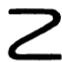
\includegraphics[keepaspectratio]{images/part001_ec6127c7.jpg}}

\begin{enumerate}
\def\labelenumi{\arabic{enumi})}
\setcounter{enumi}{1}
\item
  设 \(\mathbf{F}\) 是一个局部凸空间，它是一个递增向量子空间序列 \((\mathbf{F}_n)\) 的并，且对每个指标 \(n\) ，设 \(\mathcal{T}_n\) 是在 \(\mathbf{F}_n\) 上由拓扑 \(\mathcal{T}\) （\(\mathbf{F}\) 的）诱导的拓扑。应当注意，一般说来 \(\mathcal{T}\) 并不是诸 \(\mathcal{T}_n\) 的归纳极限。
\item
  假设 \(\mathbf{E}\) 是序列 \((\mathbf{E}_n)\) 的严格归纳极限；若 \(\mathbf{F}\) 是一个（在 \(\mathcal{T}\) 中）闭的、含于 \(\mathbf{E}\) 的向量子空间，则诸 \(\mathcal{T}_n\) 在 \(\mathrm{F} \cap \mathrm{E}_n\) 上诱导的拓扑的严格归纳极限可能严格地比 \(\mathcal{T}\) 诱导的拓扑细 (IV, 第 63 页, exerc. 10)。
\end{enumerate}

命题 10. --- 设 E, F 是两个局部凸空间。假设：

\begin{enumerate}
\def\labelenumi{\arabic{enumi})}
\item
  存在一族 Fréchet 空间 \((\mathbf{E}_{\alpha})\) ，且对每个 \(\alpha\) 有一个线性映射 \(g_{\alpha}: \mathbf{E}_{\alpha} \to \mathbf{E}\) ，使得 \(\mathbf{E}\) 的拓扑是族 \((g_{\alpha})\) 的终局部凸拓扑。
\item
  存在一个 Fréchet 空间序列 \((\mathbf{F}_n)\) ，且对每个 \(n\) 有一个连续线性单射 \(j_n: \mathbf{F}_n \to \mathbf{F}\) ，使得 \(\mathbf{F} = \bigcup j_n(\mathbf{F}_n)\) 。
\end{enumerate}

那么，每个线性映射 \(u\) （\(\mathbf{E}\) 到 \(\mathbf{F}\) 中的），只要其图在 \(\mathbf{E} \times \mathbf{F}\) 中为闭，必然连续。

为证 u 连续，只须证明对每个 \(\alpha\) ，映射 \(u \circ g_{\alpha}: E_{\alpha} \to F\) 连续 (II, 第 27 页, prop. 5)。而 \(u \circ g_{\alpha}\) 的图是 u 的图在连续映射 \(g_{\alpha} \times 1_{F}: E_{\alpha} \times F \to E \times F\) 下的逆像，因而由假设在 \(E_{\alpha} \times F\) 中是闭的。因此我们可以限于 E 本身是 Fréchet 空间的情形。但这时命题是 I, 第 20 页, prop. 1 的一个特殊情形。

推论. --- 在与 prop. 10 中关于 E 和 F 的相同假设下，并假设 E 是 Hausdorff 的，则 F 到 E 上的每个连续满射 v 是一个严格态射。

设 N 是 v 的核，并记 \(\mathrm{N}_{n}=j_{n}^{-1}(\mathrm{N})\) ；则映射 \(j_{n}^{\prime}:F_{n}/N_{n}\to F/N\) （由 \(j_{n}\) 取商得到）是单射且连续，又 \(F_{n}/N_{n}\) 是一个 Fréchet 空间（因为 \(N_{n}\) 是闭的），且 F/N 是诸 \(j_{n}^{\prime}\) 的像的并。由假设，在典范分解 \(v:F\to F/N\stackrel{w}{\to}E\) 中，线性映射 w 是双射且连续，因而其图在 \((\mathrm{F/N})\times\mathrm{E}\) 中是闭的 (GT, I, §8.1, prop. 2 的 cor. 2)。由开头的注记及 prop. 10，w 的逆映射 u 因此连续，推论得证。

* prop. 10 及其推论特别适用于如下情形：E 是一个完备的有界型空间 (III, 第 12 页)，而 F 是一个 Fréchet 空间序列的归纳极限。*

\subsection{关于 Fréchet 空间的注记}

我们将就局部凸空间的情形考虑 GT, IX, § 3.1 的 prop. 2。

命题 11. --- 设 E 是一个可度量化局部凸空间。E 的拓扑可由一个平移不变的距离定义，且对这个距离开球都是凸的。

设 \((p_{n})_{n\in\mathbf{N}}\) 是定义 E 的拓扑的一个半范数序列。设 \(d_{n}\) 是由 \(d_{n}(x,y)=\inf(p_{n}(x-y),1/n)\) （对 E 中的 x, y）定义的伪度量；它是平移不变的。对每个 \(n\geqslant0\) 及每个实数 \(R\geqslant0\) ，设 \(B_{n,R}\) 是由那些 \(x\in E\) （它们使 \(d_{n}(x,0)<R\) ）组成的集。若 \(R\geqslant1/n\) ，则 \(B_{n,R}=E\) ，而在另一情形，\(B_{n,R}\) 由那些 \(x\in E\) （它们满足 \(p_{n}(x)<R\) ）组成；在所有情形下 \(B_{n,R}\) 都是凸的。

对 \(x, y\) （\(\mathbf{E}\) 中的）定义 \(d(x, y) = \sup_{n \in \mathbb{N}} d_n(x, y)\) 。我们立即看出 \(d\) 是 \(\mathbf{E}\) 上平移不变且定义 \(\mathbf{E}\) 的拓扑的一个距离。对 \(x_0 \in \mathbf{E}\) 及 \(\mathbf{R} \geqslant 0\) ，以 \(x_0\) 为中心、\(\mathbf{R}\) 为半径的开球（对距离 \(d\) ）等于 \(\bigcap_{n \in \mathbb{N}} (x_0 + B_{n,\mathbf{R}})\) ，因此它是凸的。

命题 12. --- 设 E 和 F 是两个 Fréchet 空间，u 是 E 到 F 上的一个连续线性映射。则存在 u 的一个截面，它连续但未必线性。

由 prop. 11，存在 E 上平移不变、定义 E 的拓扑且使开球为凸的一个距离 d。给定 F 中的 y 和 \(y'\) ，设 \(\delta(y, y')\) 是闭集 \(u^{-1}(y)\) 与 \(u^{-1}(y')\) 在 E 中之间的距离。由于 u 是一个严格态射 (I, 第 17 页, th. 1)，GT, IX, §3.1 的注记表明 \(\delta\) 是 F 上定义 F 的拓扑的一个距离。我们将归纳地构造 F 到 E 中的连续映射的一个序列 \((s_n)_{n \in \mathbf{N}}\) ，使对所有 \(y \in F\) 满足下列不等式：

\[
\delta (y, u (s _ {n} (y))) <   2 ^ {- n}\tag{2}
\]

\[
d \left(s _ {n} (y), s _ {n - 1} (y)\right) <   2 ^ {- n + 1} \quad (\text { only   if } n \geqslant 1).\tag{3}
\]

于是假设或者 \(n = 0\) ，或者 \(n \geqslant 1\) 且 \(s_{n-1}\) 已经构造好。设 \(y_0 \in \mathbf{F}\) ；由于 \(u\) 是满射，集 \(u^{-1}(y_0)\) 非空，且对 \(n \geqslant 1\) ，由归纳假设有 \(d(u^{-1}(y_0), s_{n-1}(y_0)) < 2^{-n+1}\) 。因此存在一点 \(x_0\) （\(\mathbf{E}\) 中的），使 \(u(x_0) = y_0\) ，且对 \(n \geqslant 1\) ，\(d(x_0, s_{n-1}(y_0)) < 2^{-n+1}\) 。由于映射 \(s_{n-1}\) 连续，由那些点 \(y\) （\(\mathbf{F}\) 中的，满足不等式 \(\delta(y, y_0) < 2^{-n}\) 和 \(d(x_0, s_{n-1}(y)) < 2^{-n+1}\) ）所成的集是 \(y_0\) 的一个开邻域。因此存在一个开覆盖 \((\mathrm{V}_i)_{i \in \mathbf{I}}\) （\(\mathbf{F}\) 的）以及常值映射 \(s_{n,i}\) （\(\mathbf{F}\) 到 \(\mathbf{E}\) 中的），它们在 \(\mathrm{V}_i\) 中满足不等式 (2) 和 (3)（把其中的 \(s_n\) 换成 \(s_{n,i}\) ）。由于空间 \(\mathbf{F}\) 可度量化，存在一个连续的单位分解 \((f_i)_{i \in \mathbf{I}}\) ，它局部有限且从属于覆盖 \((\mathrm{V}_i)_{i \in \mathbf{I}}\) (GT, IX, § 4.5, th. 4 及 § 4.4, cor. 1)。对每个 \(y \in \mathbf{F}\) ，令 \(s_n(y) = \sum_{i \in \mathbf{I}} f_i(y) \cdot s_{n,i}(y)\) 。映射 \(s_n\) （\(\mathbf{F}\) 到 \(\mathbf{E}\) 中的）连续；由于开球在 \(\mathbf{E}\) 中和 \(\mathbf{F}\) 中都是凸的，映射 \(s_n\) 对所有 \(y \in \mathbf{F}\) 满足不等式 (2) 和 (3)。

由不等式 (3)，诸映射 \(s_n: \mathrm{F} \to \mathrm{E}\) 对一致收敛构成一个 Cauchy 序列。由于 \(\mathrm{E}\) 完备，序列 \((s_n)_{n \in \mathbb{N}}\) 一致收敛到一个连续映射 \(s: \mathrm{F} \to \mathrm{E}\) (GT, X, § 1.6)；公式 (2) 表明 \(u \circ s\) 是 \(\mathrm{F}\) 的恒等映射，因此 \(s\) 是 \(u\) 的一个连续截面。

推论. --- 若 L 是 F 中的一个紧集，则存在 E 中的一个紧集 K，使得 \(u(\mathbf{K}) = \mathbf{L}\) 。

只须取 K = s(L)，其中 s 是 u 的一个连续截面。

注记. --- 1) prop. 12 的推论也可以由 I, 第 17 页的 th. 1 及 GT, IX, § 2.10 的 prop. 18 推出。

\begin{enumerate}
\def\labelenumi{\arabic{enumi})}
\setcounter{enumi}{1}
\tightlist
\item
  我们沿用 prop. 12 的记号。设 \(p\) 是 \(E\) 上的一个连续半范数；
\end{enumerate}

对所有 \(y \in \mathbf{F}\) ，令 \(q(y) = \inf_{u(x) = y} p(x)\) ，则 \(q\) 是 \(\mathbf{F}\) 上的一个连续半范数 (II, 第 4 页)。设 \(\phi\) 是 \(F\) 到区间 \([0, +\infty[\) （\(\overline{\mathbf{R}}\) 的）中的一个下半连续映射。我们证明，存在一个连续截面 \(s\) （\(u\) 的），使得 \(p \circ s < q + \phi\) 。

设 \(s_0\) 是 \(u\) 的一个连续截面 (prop. 12)，\(\mathbf{N}\) 是 \(u\) 的核。设 \(y_0 \in \mathbf{F}\) ，则存在 \(z_0 \in \mathbf{N}\) ，使 \(p(s_0(y_0) + z_0) < q(y_0) + \phi(y_0)\) 。存在一个开邻域 \(\mathbf{W}\) （\(y_0\) 在 \(\mathbf{F}\) 中的），使 \(p(s_0(y) + z_0) < q(y) + \phi(y)\) （对所有 \(y \in \mathbf{W}\) ）。于是存在一个开覆盖 \((\mathbf{W}_i)_{i \in \mathbf{I}}\) （\(\mathbf{F}\) 的）以及常值映射 \(t_i: \mathbf{F} \to \mathbf{N}\) ，使 \(p(s_0(y) + t_i(y)) < q(y) + \phi(y)\) （对所有 \(y \in \mathbf{W}_i\) ）。由于 \(\mathbf{F}\) 可度量化，存在从属于覆盖 \((\mathbf{W}_i)_{i \in \mathbf{I}}\) 的一个局部有限的连续单位分解 \((g_i)_{i \in \mathbf{I}}\) (GT, IX, § 4.5, th. 4 及 § 4.4, cor. 1)。映射 \(s\) （\(\mathbf{F}\) 到 \(\mathbf{E}\) 中的），由 \(s(y) = s_0(y) + \sum_{i \in \mathbf{I}} g_i(y). t_i(y)\) 定义，满足所述条件。

\section{凸集的分离}

\subsection{Hahn-Banach 定理（几何形式）}

定理 1（Hahn-Banach）. --- 设 A 是拓扑向量空间 E 的一个非空开凸集，M 是一个不与 A 相交的非空线性流形。则存在一个闭超平面 H，它包含 M 且不与 A 相交。

经平移，问题可化为 \(0 \in A\) 的情形，从而 A 是吸收的。设 p 是 A 的度规 (II, 第 20 页)，于是 A 是由那些点 \(x \in E\) （它们使 \(p(x) < 1\) ）所成的集。另一方面，设 V 是由 M 生成的 E 的向量子空间；于是 M 是 V 中一个不含 0 的超平面，因而存在 V 上唯一的线性型 f，使 M 是由那些点 \(y \in V\) （它们满足 \(f(y) = 1\) ）所成的集。于是假设 \(M \cap A = \varnothing\) 蕴含对所有 \(y \in V\) （使 \(f(y) = 1\) ），有 \(p(y) \geqslant 1\) ；由于 f 和 p 都是正齐次的，\(f(y) \leqslant p(y)\) （对所有 \(y \in V\) 满足 \(f(y) > 0\) ） ；最后，由于 \(p(y) \geqslant 0\) （对所有 \(y \in V\) ），我们看出 \(f(y) \leqslant p(y)\) （对所有 \(y \in V\) ）。由 Hahn-Banach 定理的解析形式 (II, 第 22 页, th. 1)，存在 E 上的一个线性型 h，它扩张 f 且使对所有 \(x \in E\) 有 \(h(x) \leqslant p(x)\) 。设 H 是 E 中方程为 \(h(x) = 1\) 的超平面。显然 \(H \cap V = M\) 且 \(H \cap A = \varnothing\) 。另一方面，H 在 E 中的余集包含非空开集 A，因此 H 在 E 中是闭的 (I, 第 11 页, 推论)。

证毕。

注记. --- 1) 当 \(0 \in \mathbf{M}\) 时，th. 1 可陈述如下：存在 E 中的一个连续线性型，使在 M 中 \(g(x) = 0\) 而在 A 中 \(g(x) > 0\) (II, 第 8 页, prop. 4)。

\begin{enumerate}
\def\labelenumi{\arabic{enumi})}
\setcounter{enumi}{1}
\tightlist
\item
  若把定理 1 应用于 E 带有最细局部凸拓扑的情形 (II, 第 25 页, 例 2)，并且为简单起见假设 \(0 \in A\) ，则得到下面的结果（表面上不涉及拓扑）：若 A 是实向量空间 E 中的一个吸收凸集，且 M 是一个不与 A 相交的非空线性流形，则存在一个包含 M 的超平面 H，使 A 位于 H 的一侧。这个结果并非对每个凸集 A 都成立 (II, 第 65 页, exerc. 5)。
\end{enumerate}

\subsection{拓扑向量空间中凸集的分离}

定义 1. --- 实拓扑向量空间 E 的两个非空集 A, B 称为被一个闭超平面 H 分离，如果 A 含于 H 所确定的一个闭半空间中，而 B 含于另一个闭半空间中。

定义 2. --- 实拓扑向量空间的两个非空集 A, B 称为被闭超平面 H 严格分离，如果 A 含于 H 所确定的一个开半空间中，而 B 含于另一个开半空间中。

命题 1. --- 设 A 是一个非空开凸集，B 是实拓扑向量空间 E 中的一个非空凸集；若 A 不与 B 相交，则存在一个把 A 与 B 分离的闭超平面。

因为集 \(\mathbf{C} = \mathbf{A} - \mathbf{B}\) 是开的、凸的 (II, 第 9 页, prop. 7) 且非空，又有 \(0 \notin \mathbf{C}\) 。由 II, 第 36 页的定理 1，存在一个连续线性型 \(f \neq 0\) （\(\mathbf{E}\) 上的），使 \(f(z) > 0\) （在 \(\mathbf{C}\) 中） 。于是，对所有 \(x \in \mathbf{A}\) 及 \(y \in \mathbf{B}\) ，有 \(f(x) > f(y)\) 。记 \(\alpha = \inf_{x \in \mathbf{A}} f(x)\) ；\(\alpha\) 是有限的，且 \(f(x) \geqslant \alpha\) （对所有 \(x \in \mathbf{A}\) ），\(f(y) \leqslant \alpha\) （对所有 \(y \in \mathbf{B}\) ） ；闭超平面 \(\mathbf{H}\) （方程为 \(f(z) = \alpha\) ）把 \(\mathbf{A}\) 与 \(\mathbf{B}\) 分离。

注记. --- 1) 超平面 H 不与 A 相交 (II, 第 15 页, prop. 1；若 A 和 B 是两个互不相交的非空开凸集，则存在一个把 A 与 B 严格分离的闭超平面。

2) 然而，当 B 不是开集时，未必存在把 A 与 B 严格分离的闭超平面，即使 E 是有限维的，甚至即使 \(\overline{A}\) 不与 \(\overline{B}\) 相交 (II, 第 78 页, exerc. 12)。

定义 3. --- 对向量空间 E 的一个子集 A，超平面 H 称为 A 的支撑超平面，如果 H 至少包含 A 的一点，且 A 的所有点都位于 H 的同一侧。

设 f 是 E 上一个不恒为零的线性型；说方程为 \(f(x) = \alpha\) 的超平面是 A 的一个支撑超平面，意味着 \(\alpha\) 是集 \(f(A) \subset R\) 的最小元或最大元。换言之，存在 A 的一个平行于方程 \(f(x) = 0\) 的超平面的支撑超平面，必须且只需集 \(f(A)\) 的两个界之一有限且属于 \(f(A)\) 。

命题 2. --- 设 A 是拓扑向量空间 E 的一个非空紧子集。对 E 中每个闭超平面 H，存在 A 的一个平行于 H 的支撑超平面。

因为，若 \(f(x) = \gamma\) 是 H 的一个方程，其中 f 是 E 中的一个连续线性型，则 f 在 A 上的限制连续，因而有界且在 A 上达到其界 (GT, IV, § 6.1, th. 1)。

这表明存在一个或两个平行于 H 的 A 的支撑超平面；第一种情形只能在 A 完全含于一个平行于 H 的超平面时出现。

命题 3. --- 在拓扑向量空间 E 中，设 A 是一个内部非空的闭凸集。则 \(\mathbf{A}\) 的每个支撑超平面都是闭的，且 \(\mathbf{A}\) 的每个边界点都属于 \(\mathbf{A}\) 的至少一个支撑超平面。

A 的每个支撑超平面都是闭的，因为 A 的所有点都位于超平面的同一侧 (II, 第 15 页, prop. 17)。又若 \(x_0\) 是 A 的一个边界点，则 \(x_0\) 不属于非空开凸集 \(\mathring{\mathrm{A}}\) ；由 II, 第 36 页的 th. 1，存在一个包含 \(x_0\) 且不与 \(\mathring{\mathrm{A}}\) 相交的超平面 H。由于 A 是 \(\mathring{\mathrm{A}}\) 的闭包 (II, 第 14 页, prop. 16 的 cor. 1)，由 II, 第 15 页的 prop. 17 推出 H 是 A 的一个支撑超平面。

\subsection{局部凸空间中凸集的分离}

命题 4. --- 设 A 是局部凸空间 E 中的一个非空闭凸集，K 是 E 中一个不与 A 相交的非空紧凸集。则存在一个把 A 与 K 严格分离的闭超平面 H。

因为存在 E 中 0 的一个开凸邻域 V，使 A + V 与 K + V 不相交 (GT, II, § 4.3, prop. 4)。由于 A + V 与 K + V 在 E 中是凸的且开的，II, 第 37 页的 prop. 1 表明存在一个把 A + V 与 K + V 严格分离的闭超平面 H，从而更是把 A 与 K 严格分离。

注记. --- 在 Hausdorff 局部凸空间 E 中，设 A 和 B 是两个不相交的非空闭凸集，若 E 是有限维的，则存在一个把 A 与 B 分离的闭超平面 (II, 第 78 页, exerc. 13)；但当 E 是无限维时，这个结论未必成立 (II, 第 78 页, exerc. 10 及 11)。

推论 1. --- 在局部凸空间中，每个闭凸集 A 是包含它的诸闭半空间的交。

事实上，对每一点 \(x \notin \mathbf{A}\) ，存在一个把 \(x\) 与 \(\mathbf{A}\) 严格分离的闭超平面（用 prop. 4）。

推论 2. --- 在 Hausdorff 局部凸空间中，每个紧凸集 A 是包含它且由 A 的支撑超平面确定的诸闭半空间的交。

因为，设 \(x_{0} \notin A\) ；\(\{x_{0}\}\) 是闭的，因此存在一个把 \(x_{0}\) 与 A 严格分离的闭超平面 H (prop. 4)；设 \(f(x) = \alpha\) 是 H 的一个方程（f 为连续线性型），并设 \(f(x) > \alpha\) （对所有 \(x \in A\) ）。若令 \(\gamma = \inf_{x \in A} f(x)\) ，则由 \(f(x) \geqslant \gamma\) 定义的半空间包含 A，由方程为 \(f(x) = \gamma\) 的支撑超平面确定，且不含 \(x_{0}\) ；推论得证。

在局部凸空间中，一个既非紧又无内点的闭凸集可能没有任何闭的支撑超平面 (II, 第 86 页, exerc. 18：另参见 V, 第 71 页, exerc. 11)。

推论 3. --- 在局部凸空间中，每个线性流形 M 的闭包是包含 M 的诸闭超平面的交。

对所有 \(x \notin \overline{\mathbf{M}}\) ，设 \(\mathbf{H}\) 是一个把 \(x\) 与 \(\overline{\mathbf{M}}\) 严格分离的闭超平面；

于是 \(\overline{M}\) 平行于 H；闭超平面 \(H_{1}\) （包含 \(\overline{M}\) 且平行于 H 的）不含 x。推论得证。

推论 4. --- 设 C 是局部凸空间 E 中的一个闭凸集。E 的子集 A 含于 C，必须且只需对 E 上每个使得对所有 C 中的 x 有 \(u(x) \geqslant 0\) 的实值连续仿射函数 u，都有对所有 A 中的 y，\(u(y) \geqslant 0\) 。

条件显然是必要的。反之我们证明它是充分的；若一点 \(x \in A\) 不含于 C，则存在一个方程为 \(f(z) = \alpha\) 的闭超平面把 x 与 C 严格分离；若例如设 \(f(x) < \alpha\) ，则连续仿射函数 \(u = f - \alpha\) 与假设矛盾。

推论 5. --- 在局部凸空间 E 中，每个以 0 为顶点的凸锥 C 的闭包是包含 C 且由过 0 的闭超平面确定的诸闭半空间的交。

因为 \(\overline{\mathbf{C}}\) 是一个以 0 为顶点的凸锥 (II, 第 13 页, prop. 14)。对 \(x \notin \overline{\mathbf{C}}\) ，存在一个把 \(x\) 与 \(\overline{\mathbf{C}}\) 严格分离的闭超平面 H (prop. 4)。这时只须应用下面的引理：

引理 1. --- 若一个以 0 为顶点的锥 A 含于由超平面 H 确定的一个开半空间中，则它含于由一个平行于 H 且过 0 的超平面 \(H_{0}\) 确定的闭半空间中。

设 \(f(z) = \alpha\) （\(\alpha < 0\) ）是 H 的一个方程，于是 \(f(z) = 0\) 是 \(H_0\) 的方程。若存在 \(z \in A\) 使 \(f(z) < 0\) ，则将存在 \(\lambda > 0\) 使 \(f(\lambda z) = \alpha\) ，而由于 \(\lambda z \in A\) ，这将与假设矛盾。

\subsection{凸函数的逼近}

命题 5. --- 设 X 是局部凸空间 E 中的一个闭凸集。则每个在 X 上定义的下半连续凸函数 f 都是 E 中连续仿射线性函数限制到 X 上所得函数组成的一个族的上包络。

因为，集 \(A \subset E \times R\) （它由那些点 \((x, t)\) 组成：\(x \in X\) 且 \(t \geqslant f(x)\) ）是凸的 (II, 第 17 页, prop. 19) 且闭的，因为函数 \((x, t) \mapsto f(x) - t\) 是下半连续的。设 x 是 X 的任一点，且设 \(a \in R\) 满足 \(a < f(x)\) 。由 II, 第 38 页的 cor. 1，存在 \(E \times R\) 中的一个闭超平面 H，它包含 \((x, a)\) 且不与 A 相交。由于 \(E \times R\) 上每个连续线性型都形如

\[
(z, t) \rightarrow u (z) + \lambda t,
\]

其中 \(\lambda\in R\) 而 u 是 E 上的一个连续线性型，由此可知 H 有形如 \(u(z)+\lambda t=\alpha\) 的方程，且由于 H 包含 \((x,a)\) ，我们有 \(\alpha=u(x)+\lambda a\) 。而点 \((x,f(x))\in\mathbf{A}\) 不属于 H，因此 \(\lambda\neq0\) 。必要时除以 \(-\lambda\) ，可把 H 的方程写成 \(t-a=u(z-x)\) 。由于 \(f(x)-a>0\) ，我们有 \(f(z)>u(z-x)+a\) （对所有 \(z\in X\) ），这就证明了命题。

注记. --- 1) 由 prop. 5 推出，f 是一个递增有向函数族的上包络，该族的函数是 E 中连续且凸的函数限制到 X 上的限制。

\begin{enumerate}
\def\labelenumi{\arabic{enumi})}
\setcounter{enumi}{1}
\tightlist
\item
  进一步假设 X 是一个以 0 为顶点的闭凸锥，且 f 是正齐次的。则 f 是 E 中连续线性型限制到 X 上所得函数组成的一个族的上包络。因为，设 \((u_{\alpha})\) 是 E 中连续仿射线性函数组成的一个族，它们在 X 上的限制以 f 为上包络。记 \(u_{\alpha} = v_{\alpha} + \lambda_{\alpha}\) ，其中 \(\lambda_{\alpha} \in R\) ，而 \(v_{\alpha}\) 是 E 中的一个连续线性型。我们有 \(\lambda_{\alpha} = u_{\alpha}(0) \leqslant f(0) = 0\) 。另一方面，若 \(x \in X\) ，则对每个 \(\mu > 0\) 有
\end{enumerate}

\[
\mu^ {- 1} \lambda_ {\alpha} + v _ {\alpha} (x) = \mu^ {- 1} (\lambda_ {\alpha} + v _ {\alpha} (\mu x)) = \mu^ {- 1} u _ {\alpha} (\mu x) \leqslant \mu^ {- 1} f (\mu x) = f (x)
\]

因此在 X 中 \(u_{\alpha} \leqslant v_{\alpha} \leqslant f\) ，从而 \(f\) 是诸 \(v_{\alpha}\) 的上包络。

\begin{enumerate}
\def\labelenumi{\arabic{enumi})}
\setcounter{enumi}{2}
\tightlist
\item
  E 中连续仿射函数在 X 上的限制是 X 上的一个仿射函数（即既凹又凸，II, 第 17 页）；但可能发生这样的情形：在紧凸集 \(\mathbf{X} \subset \mathbf{E}\) 中存在连续仿射函数，它们不是 E 中连续仿射函数在 X 上的限制 (II, 第 78 页, exerc. II, c))。然而：
\end{enumerate}

命题 6. --- 设 f 是 Hausdorff 局部凸空间 E 的紧凸集 X 上的一个上半连续仿射函数。设 L 是 E 中连续仿射函数在 X 上的限制所成的集；则由那些 \(h \in L\) （它们满足 \(h(x) > f(x)\) ，对所有 \(x \in X\) ）组成的集 L' 是递减有向的，且其下包络等于 f。

我们可以假设 X 非空。设 u, v 是 L 的两个元，使得 \(u(x) > f(x)\) 且 \(v(x) > f(x)\) （对所有 \(x \in X\) ），并设 b 是 u 和 v 的一个上界常数。设 U（相应地 V）是由点 \((x, t)\) （在 \(X \times R\) 中满足 \(u(x) \leqslant t \leqslant b\) （相应地 \(v(x) \leqslant t \leqslant b\) ））所成的紧凸集，并设 F 是由 \((x, t) \in X \times R\) （满足 \(t \leqslant f(x)\) ）所成的集；F 在 \(X \times R\) 中是凸的且闭的。\(U \cup V\) 的凸包 K 不与 F 相交，因为 \(U \cup V\) 含于由 \((x, t) \in X \times R\) （满足 \(f(x) < t\) ）所成的集中，而后者是凸的且不与 F 相交。由于 K 是紧的 (II, 第 14 页, prop. 15)，我们可以用 \(E \times R\) 中的一个闭超平面 H 把 F 与 K 严格分离。对每个 \(x \in X\) ，超平面 H 把 \((x, f(x))\) 与 \((x, b)\) 严格分离，因此与直线 \(\{x\} \times R\) 交于单独一点 \(w(x)\) ；于是 H 是一个连续仿射函数的图象，其在 X 上的限制 w 属于 L，是 u 和 v 的一个下界，且满足不等式 \(w(x) > f(x)\) （对所有 \(x \in X\) ）。这就证明集 \(L'\) 是递减有向的。把 II, 第 39 页的 prop. 5 应用于 -f，可知 f 是 \(L'\) 的下包络。

推论. --- 设 \(f\) 是 \(\mathbf{X}\) 中的一个连续仿射函数；则存在一个序列 \((h_n)\) （由 \(\mathbf{L}\) 的元素组成），它一致收敛于 \(f\) （在 \(\mathbf{X}\) 中） 。

因为，prop. 6 与 Dini 定理 (GT, X, § 4.1, th. 1) 表明，对所有 \(n\) 存在 \(h_n \in \mathbf{L}\) 使 \(f \leqslant h_n \leqslant f + 1/n\) 。

\section{弱拓扑}

\subsection{对偶向量空间}

设 \(\mathbf{F}\) 和 \(\mathbf{G}\) 是两个实向量空间，\((x, y) \mapsto \mathbf{B}(x, y)\) 是 \(\mathbf{F} \times \mathbf{G}\) 上的一个双线性型。我们说双线性型 \(\mathbf{B}\) 使向量空间 \(\mathbf{F}\) 和 \(\mathbf{G}\) 成对偶，或说 F 和 G 成对偶（关于 B）。回忆我们称 \(x \in F\) 和 \(y \in G\) （对由 B 定义的对偶）正交，如果 \(\mathbf{B}(x, y) = 0\) ；我们称 F 的一个子集 M 和 G 的一个子集 N 正交，如果每个 \(x \in M\) 与每个 \(y \in N\) 都正交 (A, IX, § 1.2)。

我们说由 B 定义的对偶在 F 中（相应地在 G 中）分离，如果它满足下列条件：

(D₁) 对 F 中每个 \(x \neq 0\) ，存在 \(y \in G\) 使 \(\mathrm{B}(x, y) \neq 0\) 。（相应地 (D \(_{II}\) ) 对 G 中每个 y ≠ 0，存在 x ∈ F 使 B(x, y) ≠ 0。）

由 B 定义的对偶称为分离的，如果它在 F 中和 G 中都分离。为此，必须且只需双线性型 B 在 A, IX, § 1.1 的意义下是分离的。更精确地，我们有下面的结果：

命题 1. --- 设 F, G 是两个实向量空间，B 是 F × G 上的一个双线性型。设

\[
d _ {\mathrm{B}}: y \mapsto \mathrm{B} (., y),
\]

\[
s _ {\mathbf {B}} \colon x \mapsto \mathrm{B} (x,.)
\]

分别是 G 到 F 的对偶 F* 中和 F 到 G 的对偶 G* 中的线性映射，它们分别伴随于 B 的右与左 (A, IX, § 1.1)。则 B 使 F 和 G 成一个在 G 中（相应地在 F 中）分离的对偶，必须且只需 \(d_{\mathbf{B}}\) （相应地 \(s_{\mathbf{B}}\) ）是单射。

当 F 和 G 被 B 置于分离对偶时，我们常把 F（相应地 G）等同于 \(G^{*}\) （相应地 \(F^{*}\) ）的一个子空间（借助 \(s_{B}\) （相应地 \(d_{B}\) ））。当我们把 F（相应地 G）看作 \(G^{*}\) （相应地 \(F^{*}\) ）的一个子空间而不指明这个等同如何实现时，我们总是在使用前述的等同；这时双线性型 B 等同于典范双线性型在 \(F \times G\) 上的限制：

\[
(x ^ {*}, x) \mapsto \langle x, x ^ {*} \rangle \quad (\text { resp. } (x, x ^ {*}) \mapsto \langle x, x ^ {*} \rangle).
\]

例. --- 1) 设 E 是一个向量空间，E* 是它的对偶。典范双线性型 \((x, x^{*}) \mapsto \langle x, x^{*} \rangle\) （\(E \times E^{*}\) 上的）(A, II, §2.3) 使 E 和 \(E^{*}\) 成分离对偶：因为 \((\mathrm{D}_{\mathrm{II}})\) 由关系 \(x^{*} \neq 0\) 的定义得出，另一方面我们知道，对 E 中所有 \(x \neq 0\) ，存在线性型 \(x^{*} \in E^{*}\) 使 \(\langle x, x^{*} \rangle \neq 0\) (A, II, §7.5, th. 6)，这就证明了 \((\mathrm{D}_{\mathrm{I}})\) ；这里 E 与 \(E^{**}\) 的一个子空间的等同由典范映射 \(c_{E}\) 实现 (loc. cit.)。

当 E 是有限维时，与 E 成分离对偶的 \(E^{*}\) 的子空间 G（借助典范双线性型在 \(E \times G\) 上的限制）只有 \(E^{*}\) 自身；因为这时 E 典范地等同于 \(E^{**}\) (loc. cit.)，倘若有 \(G \neq E^{*}\) ，就将存在 E 中的 \(a \neq 0\) ，使 \(\langle a, x^{*} \rangle = 0\) （对所有 \(x^{*} \in G\) ） (A, II, §7.5, th. 7)，这与假设矛盾。

\begin{enumerate}
\def\labelenumi{\arabic{enumi})}
\setcounter{enumi}{1}
\tightlist
\item
  当 E 是无限维向量空间且 \(E'\) 是 \(E^{*}\) 的一个向量子空间时，E 与 \(E'\) 之间的对偶（由典范双线性型在 \(E \times E'\) 上的限制所定义）总是在 \(E'\) 中分离的；即使 \(E' \neq E^{*}\) ，它也可以在 E 中分离。最重要的情形是 E 为拓扑向量空间的情形。
\end{enumerate}

定义 1. --- 拓扑向量空间 E 的对偶指的是向量空间 E 的对偶 E* 中由 E 上的连续线性型组成的子空间 E'。

当 E 是 Hausdorff 局部凸空间时，E 与其对偶 \(E'\) 之间的对偶是分离的：这由 Hahn-Banach 定理 (II, 第 24 页, cor. 1) 得出，即对 E 中每个 \(x \neq 0\) ，存在 \(x' \in E'\) 使 \(\langle x, x' \rangle \neq 0\) 。

注记. --- 1) 当 E 是拓扑向量空间时，向量空间 E 的对偶 E* 将称为 E 的代数对偶，以避免混淆。我们还注意，E* 是给 E 赋予最细局部凸拓扑 (II, 第 25 页, 例 2) 后所得拓扑向量空间的对偶。

\begin{enumerate}
\def\labelenumi{\arabic{enumi})}
\setcounter{enumi}{1}
\item
  拓扑向量空间的对偶 \(\mathbf{E}'\) 本身不带有拓扑，除非明确声明。
\item
  若 \(\mathbf{F}\) 与 \(\mathbf{G} \subset \mathbf{F}^*\) 由典范双线性型成分离对偶，则 \(\mathbf{F}\) 与 \(\mathbf{G}_1\) 也成分离对偶，对子空间 \(\mathbf{G}_1\) （\(\mathbf{F}^*\) 的，满足 \(\mathbf{G} \subset \mathbf{G}_1\) ）。
\end{enumerate}

\subsection{弱拓扑}

定义 2. --- 设 F 和 G 是由双线性型 B 置于对偶的两个向量空间。F 上使所有线性型 \(\mathbf{B}(., y): x \mapsto \mathbf{B}(x, y)\) （其中 y 取遍 G）都连续的最粗拓扑，称为由 F 与 G 之间的对偶定义的 F 上的弱拓扑，我们把它记作 \(\sigma(\mathbf{F}, \mathbf{G})\) 。

类似地，我们定义弱拓扑 \(\sigma(\mathbf{G},\mathbf{F})\) （\(\mathbf{G}\) 上的；在定义 1 中交换 \(\mathbf{F}\) 与 \(\mathbf{G}\) ）；这种交换 \(\mathbf{F}\) 与 \(\mathbf{G}\) 的可能性适用于本节以下的所有结果和定义。

只要不会混淆，我们用形容词「弱」和副词「弱地」表示关于弱拓扑 \(\sigma(\mathrm{F},\mathrm{G})\) 的性质。例如我们将说「弱收敛」「弱连续函数」等。

当 \(G \subset F^{*}\) 时，记号 \(\sigma(F, G)\) 总表示由对应于在 \(F \times G\) 上的限制（典范双线性型 \((x, x^{*}) \mapsto \langle x, x^{*} \rangle\) 的限制）的对偶所定义的弱拓扑。

在不对 F 和 G 附加假设的情况下，只要没有歧义，我们常用 \(\langle x, y \rangle\) 表示双线性型 B 的值 \(\mathbf{B}(x, y)\) （在点 \((x, y)\) 处的）；我们在本节余下部分采用这一约定。

带有弱拓扑 \(\sigma(F, G)\) 的向量空间 F 称为弱空间。弱拓扑 \(\sigma(F, G)\) 是局部凸的 (II, 第 26 页, prop. 4)；更精确地说，它是 \(\mathbf{R}^G\) 的乘积拓扑在线性映射 \(\phi: x \mapsto (\langle x, y \rangle)_{y \in G}\) （\(F\) 到 \(\mathbf{R}^G\) 中的）下的逆像。它由半范数 \(x \mapsto |\langle x, y \rangle|\) （其中 \(y\) 取遍 \(G\) ）所成的集定义 (II, 第 5 页)。对每个 \(\alpha > 0\) 及有限族 \((y_i)_{1 \leq i \leq n}\) （\(G\) 的点的），设 \(W(y_1, ..., y_n; \alpha)\) 是由那些 \(x \in F\) （它们满足 \(|\langle x, y_i \rangle| \leqslant \alpha\) ，\(1 \leq i \leq n\) ）组成的集；这些集（对任意的 \(\alpha, n\) 和 \(y_i\) ）构成 \(\sigma(F, G)\) 下 0 的一个基本邻域系。注意 \(W(y_1, ..., y_n; \alpha)\) 包含 \(F\) 的由方程 \(\langle x, y_i \rangle = 0\) （ \(1 \leq i \leq n\) ）定义的那个有限余维数向量子空间。

命题 2. --- 弱拓扑 \(\sigma(F, G)\) 是 Hausdorff 的，必须且只需 \(F\) 与 \(G\) 之间的对偶在 \(F\) 中分离。

这是 II, 第 3 页, prop. 2 的一个特殊情形。

命题 3. --- 设 F 和 G 是两个成对偶的实向量空间。F 上每个对 \(\sigma(F, G)\) 连续的线性型都可写成 \(x \mapsto \langle x, y \rangle\) ，其中 \(y \in G\) 。当对偶在 G 中分离时，元 \(y \in G\) 是唯一的。

因为，说线性型 \(f\) （\(\mathbf{F}\) 上的）对 \(\sigma(\mathbf{F}, \mathbf{G})\) 连续，意味着存在有限多个点 \(y_i \in \mathbf{G}\) （ \(1 \leqslant i \leqslant n\) ），使对所有 \(x\) （\(\mathbf{F}\) 中的）有 \(|f(x)| \leqslant \sup_{1 \leqslant i \leqslant n} |\langle x, y_i \rangle|\) (II, 第 6 页, prop. 5)。于是 \(n\) 个关系 \(\langle x, y_i \rangle = 0\) （ \(1 \leqslant i \leqslant n\) ）蕴含 \(f(x) = 0\) ，从而 (A, II, § 7.5, cor. 1) 存在线性组合 \(y = \sum_{i=1}^{n} \lambda_i y_i\) ，使 \(f(x) = \langle x, y \rangle\) （对所有 \(x \in \mathbf{F}\) ）。唯一性由 \((\mathrm{D}_{\mathrm{II}})\) 得出。

换言之，当对偶在 G 中分离且 F 带有拓扑 \(\sigma(\mathrm{F}, \mathrm{G})\) 时，我们可以把 G 典范地等同于对这个拓扑的 F 的对偶 (II, 第 42 页, def. 1)。

推论 1. --- F 的点组成的族 \((a_i)\) 对拓扑 \(\sigma(\mathrm{F},\mathrm{G})\) 是完全的，必须且只需对 G 中每个 \(y \neq 0\) ，存在指标 \(\iota\) 使 \(\langle a_{\iota}, y \rangle \neq 0\) 。

因为利用 prop. 3 及 I, 第 13 页, th. 1，该性质表达了这样的事实：对 \(\sigma(F, G)\) 没有闭超平面包含所有 \(a_{i}\) ；于是推论由 II, 第 38 页的 cor. 3 得出。

推论 2. --- F 的点组成的族 \((a_{\iota})\) 对拓扑 \(\sigma(\mathrm{F}, \mathrm{G})\) 是拓扑无关的，必须且只需对每个指标 \(\iota\)，存在元 \(b_{\iota} \in G\) ，使 \(\langle a_{\iota}, b_{\iota} \rangle \neq 0\) 且 \(\langle a_{\kappa}, b_{\iota} \rangle = 0\) （对所有 \(\kappa \neq \iota\) ）。

这意味着，对所有 \(\iota\) ，存在 \(\sigma(F, G)\) 中的一个闭超平面，它包含所有的 \(a_{\kappa}\) （带指标 \(\kappa \neq \iota\) 的）但不含 \(a_{\iota}\) 。

推论 3. --- 设 \(G_{1}\) 和 \(G_{2}\) 是 \(F^{*}\) 的两个向量子空间，它们（对典范双线性型的限制）与 F 成对偶。则 \(\sigma(F, G_{2})\) 比 \(\sigma(F, G_{1})\) 细，必须且只需 \(G_{1} \subset G_{2}\) 。

条件显然是充分的；反之，若 \(\sigma(F, G_2)\) 比 \(\sigma(F, G_1)\) 细，则每个对 \(\sigma(F, G_1)\) 连续的线性型也对 \(\sigma(F, G_2)\) 连续，从而由 prop. 3 得 \(G_1 \subset G_2\) 。

推论 4. --- 设 G 是向量空间 F 的对偶 F* 的一个向量子空间。则 F 与 G （对典范双线性型）成分离对偶，必须且只需 G 在 F* 中对拓扑 σ(F*, F) 稠密。

这由 cor. 1 得出。

\subsection{极集与正交子空间}

定义 2. --- 设 F 和 G 是两个成对偶的（实）向量空间。对 F 的每个集 M，我们称由那些 \(y \in G\) （它们满足 \(\langle x, y \rangle \geqslant -1\) ，对所有 \(x \in M\) ）组成的集为 M 的极集。（对复向量空间，参见 II, 第 64 页。）

若 \(G_{1}\) 、 \(G_{2}\) 是 \(F^{*}\) 的两个满足 \(G_{1} \subset G_{2}\) 的子空间，则 M 在 \(G_{1}\) 中的极集是 \(G_{1}\) 与 M 在 \(G_{2}\) 中的极集的交。

当没有混淆危险时，我们用 \(M^{\circ}\) 表示 F 的子集 M 在 G 中的极集。类似地，我们定义 G 中的集在 F 中的极集。

显然，对每个标量 \(\lambda \neq 0\) 及所有 \(\mathbf{M} \subset \mathbf{F}\) ，有 \((\lambda \mathbf{M})^{\circ} = \lambda^{-1} \mathbf{M}^{\circ}\) 。关系 \(\mathbf{M} \subset \mathbf{N} \subset \mathbf{F}\) 蕴含 \(\mathbf{N}^{\circ} \subset \mathbf{M}^{\circ}\) ；若 \(\mathbf{N}\) 吸收 \(\mathbf{M}\) ，则 \(\mathbf{M}^{\circ}\) 吸收 \(\mathbf{N}^{\circ}\) ；对每个族 \((\mathbf{M}_{\alpha})\) （\(\mathbf{F}\) 的集组成的），\(\bigcup_{\alpha} \mathbf{M}_{\alpha}\) 的极集是诸极集 \(\mathbf{M}_{\alpha}^{\circ}\) 的交。由于对 \(y \in \mathbf{M}^{\circ}\) ，由关系 \(\langle x, y \rangle \geqslant -1\) 定义的闭半空间包含 0 和 \(\mathbf{M}\) ，我们看出，若 \(\mathbf{M}_{1}\) 是 \(\mathbf{M} \cup \{0\}\) 的凸包，则 \(\mathbf{M}_{1}^{\circ} = \mathbf{M}^{\circ}\) 。

显然 \(\mathbf{M} \subset \mathbf{M}^{\circ \circ}\) 。于是

\[
(\mathbf {M} ^ {\circ \circ}) ^ {\circ} \subset \mathbf {M} ^ {\circ} \subset (\mathbf {M} ^ {\circ}) ^ {\circ \circ} = (\mathbf {M} ^ {\circ \circ}) ^ {\circ}
\]

即 \(\mathbf{M}^{\circ \circ \circ} = \mathbf{M}^{\circ}\) （参见 S, III, § 1.5, prop. 2）。

若 \(\mathbf{M}\) 是 \(\mathrm{F}\) 的一个对称子集，则 \(\mathbf{M}^{\circ}\) 是 \(\mathbf{G}\) 的一个对称子集；这时 \(\mathbf{M}^{\circ}\) 也是由那些 \(y \in \mathbf{G}\) （它们满足 \(|\langle x, y \rangle| \leqslant 1\) ，对所有 \(x \in \mathbf{M}\) ）组成的集。

命题 4. --- (i) 对 F 的任一集 M，极集 \(\mathbf{M}^{\circ}\) 是一个包含 0 的凸集，且在 G 中对拓扑 \(\sigma(\mathbf{G},\mathbf{F})\) 是闭的。

\begin{enumerate}
\def\labelenumi{(\roman{enumi})}
\setcounter{enumi}{1}
\item
  若 \(\mathbf{M}\) 是一个以 0 为顶点的锥，则 \(\mathbf{M}^{\circ}\) 是一个以 0 为顶点的锥，它也是由那些 \(y\in \mathbf{G}\) （它们满足 \(\langle x,y\rangle \geqslant 0\) ，对所有 \(x\in \mathbf{M}\) ）组成的集。
\item
  若 \(\mathbf{M}\) 是 \(\mathbf{F}\) 的一个向量子空间，则 \(\mathbf{M}^{\circ}\) 是 \(\mathbf{G}\) 的一个向量子空间，它也是由那些 \(y \in \mathbf{G}\) （它们满足 \(\langle x, y \rangle = 0\) ，对所有 \(x \in \mathbf{M}\) ）组成的集。
\item
  由于线性型 \(y \mapsto \langle x, y \rangle\) 对 \(\sigma(\mathbf{G}, \mathbf{F})\) 连续，结论由定义以及由超平面确定的半空间是凸的这一事实立即得出。
\item
  若 \(\mathbf{M}\) 是一个以 0 为顶点的锥，且 \(x \in \mathbf{M}\) 、\(y \in \mathbf{M}^{\circ}\) ，则由于 \(\lambda x \in \mathbf{M}\) （对所有 \(\lambda > 0\) ），我们有 \(\langle \lambda x, y \rangle \geqslant -1\) ，即 \(\lambda \langle x, y \rangle \geqslant -1\) 。由于这对所有 \(\lambda > 0\) 成立，推出 \(\langle x, y \rangle \geqslant 0\) ，(ii) 得证。
\item
  类似地，若 \(\mathbf{M}\) 是 \(\mathbf{F}\) 的一个向量子空间，则关系 \(x \in \mathbf{M}\) 、\(y \in \mathbf{M}^{\circ}\) 这一次蕴含 \(\lambda \langle x, y \rangle \geqslant -1\) （对所有实数 \(\lambda\) ），这只有当 \(\langle x, y \rangle = 0\) 时才可能。
\end{enumerate}

若 \(\mathbf{M}\) 是 \(\mathbf{F}\) 的一个向量子空间，我们称 \(\mathbf{M}^{\circ}\) 为 \(\mathbf{M}\) 在 \(\mathbf{G}\) 中的正交（子空间）；若 \(\mathbf{G} \subset \mathbf{F}^{*}\) ，则 \(\mathbf{M}^{\circ}\) 是 \(\mathbf{G}\) 与 \(\mathbf{M}\) 在代数对偶 \(\mathbf{F}^{*}\) （\(\mathbf{F}\) 的）中的正交子空间的交 (A, II, § 2.4, def. 4)。

对 F 的向量子空间 M 和 G 的向量子空间 N，我们说 M 和 N 正交，如果 \(M \subset N^{0}\) （或者等价地，\(N \subset M^{\circ}\) ）。

定理 1（双极定理）. --- 设 F, G 是两个成对偶的实向量空间。对 F 的每个子集 M，\(M^{\circ\circ}\) ——M 在 G 中的极集 \(M^{\circ}\) 在 F 中的极集—— 是（对 \(\sigma(F, G)\) 而言）\(M \cup \{0\}\) 的闭凸包。

我们已看到，只须考虑 M 是凸的且 \(0 \in M\) 的情形。M 在拓扑 \(\sigma(F, G)\) 中的闭包记作 \(\overline{M}\) ，则 \(\overline{M}\) 是 F 中的一个凸集；II, 第 44 页的 prop. 4 表明 \(M^{\circ\circ} \supset \overline{M}\) 。另一方面，若 \(a \in F\) 不属于 \(\overline{M}\) ，则存在 F 中的一个闭超平面 H 把 a 与 \(\overline{M}\) 严格分离 (II, 第 38 页, prop. 4)；由于 H 不包含 0，存在 \(y \in G\) 使 H 有方程 \(\langle x, y \rangle = -1\) (II, 第 43 页, prop. 3)；于是 \(\langle x, y \rangle > -1\) （对所有 \(x \in \overline{M}\) ）而 \(\langle a, y \rangle < -1\) 。这蕴含 \(y \in M^{\circ}\) 且 \(a \notin M^{\circ\circ}\) ，从而关系 \(M^{\circ\circ} = \overline{M}\) 得证。

推论 1. --- 对任一族 \((\mathbf{M}_{\alpha})\) （诸集为 F 中对拓扑 \(\sigma(\mathrm{F}, \mathrm{G})\) 闭的凸集，且每个都包含 0），交 \(M = \bigcap_{\alpha} M_{\alpha}\) 的极集是（对 \(\sigma(\mathrm{G}, \mathrm{F})\) 而言）诸 \(M_{\alpha}^{\circ}\) 的并的闭凸包。

因为，若 N 是这个闭凸包，则

\[
\mathbf {N} ^ {\circ} = \bigcap_ {\alpha} \mathbf {M} _ {\alpha} ^ {\circ \circ} = \bigcap_ {\alpha} \mathbf {M} _ {\alpha} = \mathbf {M}
\]

于是 \(N = N^{\circ\circ} = M^{\circ}\) 。

若诸 \(M_{\alpha}\) 不是凸的，cor. 1 的结论未必成立。

推论 2. --- 对 F 的每个向量子空间 M，子空间 \(M^{\circ\circ}\) 是 M 在拓扑 \(\sigma(\mathrm{F}, \mathrm{G})\) 中的闭包。

注记. --- 拓扑 \(\sigma(\mathrm{G},\mathrm{F})\) 下 G 中 0 的每个邻域包含一个由有限多个形如 \(|\langle x_i,y\rangle |\leqslant 1\) （ \(1\leqslant i\leqslant n\) ）的不等式定义的邻域 V，其中 \(x_{i}\) 是 F 的任意点。若 A 是诸 \(x_{i}\) 组成的集的对称凸包，则 V 是 A 在 G 中的极集 \(\mathrm{A}^{\circ}\) 。我们可以说，F 中有限对称集（或其凸包）在 G 中的极集构成 \(\sigma(\mathrm{G},\mathrm{F})\) 下 G 中 0 的一个基本邻域系。若对偶在 F 中分离，则这些凸包对 \(\sigma(\mathrm{F},\mathrm{G})\) 是紧的 (II, 第 14 页, prop. 15 的 cor. 1) 且是有限维的。反之，F 中每个有限维紧凸集 C（带 \(\sigma(\mathrm{F},\mathrm{G})\) 拓扑）含于 F 的一个有限子集的凸包中。因为，设 M 是包含 C 的一个有限维向量子空间。若 \((e_i)_{1\leqslant i\leqslant n}\) 是 M 的一个基，我们可以假设 C 含于以 0 为中心、在基 \(e_i\) 的向量上构造的闭平行多面体中 (GT, VI, § 1.3)；而立即可见，这个平行多面体是点 \(\sum_{i=1}^{n} \varepsilon_i e_i\) （\(\varepsilon_i = \pm 1\) ）的凸包。

于是我们可以说，（若 \(\sigma(\mathrm{F},\mathrm{G})\) 是 Hausdorff 的）F 中有限维凸紧集（对 \(\sigma(\mathrm{F},\mathrm{G})\) 或对 F 上任何比 \(\sigma(\mathrm{F},\mathrm{G})\) 细的 Hausdorff 局部凸拓扑）的极集构成 \(\sigma(\mathrm{G},\mathrm{F})\) 下 0 的一个基本邻域系。

推论 3. --- 设 T 是局部凸空间 E 的拓扑，E' 是它的对偶 (II, 第 42 页, def. 1)。

\begin{enumerate}
\def\labelenumi{(\roman{enumi})}
\item
  \(\mathbf{E}\) 中的闭凸集对拓扑 \(\mathcal{T}\) 和对弱拓扑 \(\sigma (\mathrm{E},\mathrm{E}^{\prime})\) 是相同的。
\item
  对每个子集 \(\mathbf{M}\) （\(\mathbf{E}\) 的），\(\mathbf{M}^{\circ \circ}\) （在 \(\mathbf{E}\) 中；\(\mathbf{M}^{\circ}\) —— \(\mathbf{M}\) 在 \(\mathbf{E}'\) 中的极集—— 的极集）是 \(\mathbf{M} \cup \{0\}\) 对拓扑 \(\mathcal{T}\) 的闭凸包。
\end{enumerate}

显然，(ii) 由 (i) 及 th. 1 得出。由对偶 E' 的定义，II, 第 43 页的 prop. 3 表明 E 上对拓扑 T 的连续线性型与对 \(\sigma(\mathrm{E}, \mathrm{E}')\) 的连续线性型相同。因此 E 中的闭半空间对 T 和对 \(\sigma(\mathrm{E}, \mathrm{E}')\) 是相同的 (II, 第 15 页, prop. 17)，于是断言 (i) 由 II, 第 38 页的 cor. 1 得出。

\subsection{连续线性映射的转置}

在本节中，我们假设 \((\mathrm{F},\mathrm{G})\) 和 \((\mathrm{F}_1,\mathrm{G}_1)\) 是两对成对偶的向量空间。

命题 5. --- 设 u 是 F 到 \(F_{1}\) 中的一个线性映射。下列性质等价：

\begin{enumerate}
\def\labelenumi{\alph{enumi})}
\item
  \(u\) 对弱拓扑 \(\sigma (\mathrm{F},\mathrm{G})\) 和 \(\sigma (\mathrm{F}_1,\mathrm{G}_1)\) 连续；
\item
  存在一个映射 \(v: \mathbf{G}_1 \to \mathbf{G}\) 使得
\end{enumerate}

\[
\langle u (y), z _ {1} \rangle = \langle y, v (z _ {1}) \rangle\tag{1}
\]

对所有 \(y \in \mathbf{F}\) 和 \(z \in \mathbf{G}_1\) 成立。

若这些性质成立且 \(\mathbf{F}\) 与 \(\mathbf{G}\) 之间的对偶在 \(\mathbf{G}\) 中分离，则满足 (1) 的映射 \(v\) 是唯一的，且 \(v\) 是线性的。

若 u 对弱拓扑连续，则对所有 \(z_{1} \in G_{1}\) ，F 上的线性型 \(y \mapsto \langle u(y), z_{1} \rangle\) 对 \(\sigma(F, G)\) 连续，于是 (II, 第 43 页, prop. 3) 可写成 \(y \mapsto \langle y, v(z_{1}) \rangle\) ，其中 \(v(z_{1}) \in G\) ，这表明 a) 蕴含 b)。反之，若 b) 成立，则对所有 \(z_{1} \in G_{1}\) ，线性型

\[
y \mapsto \langle y, v (z _ {1}) \rangle = \langle u (y), z _ {1} \rangle
\]

对 \(\sigma(\mathrm{F},\mathrm{G})\) 连续：由弱拓扑的定义推出 \(u\) 对 \(\sigma(\mathrm{F},\mathrm{G})\) 和 \(\sigma(\mathrm{F}_1,\mathrm{G}_1)\) 连续 (I, 第 10 页, cor. 1)。\(v\) 的唯一性由 \((\mathrm{D}_{\mathrm{II}})\) 得出，而这个唯一性蕴含 \(v\) 是线性的。

注记. --- 假设 F 与 G 之间的对偶在 G 中分离，且 \(F_{1}\) 与 \(G_{1}\) 之间的对偶在 \(G_{1}\) 中分离。若我们把 G 和 \(G_{1}\) 分别等同于 \(F^{*}\) 和 \(F_{1}^{*}\) 的子空间，则条件 a) 和 b) 等价于 \(^{t}u(\mathbf{G}_{1}) \subset \mathbf{G}\) ；v 是 u 的转置 \(^{t}u\) (A, II, §2.5) 在 \(G_{1}\) 上的限制。

我们简单地（当没有混淆可能时）称 v 为 u 的转置（关于一方面 F 与 G 之间、另一方面 \(F_{1}\) 与 \(G_{1}\) 之间的对偶），并且仍用 \(^{t}u\) 记它。

推论. --- 假设 F 与 G 之间的对偶在 G 中分离。若 u 是 F 到 \(F_{1}\) 中的一个线性映射，它对 \(\sigma(F, G)\) 和 \(\sigma(F_{1}, G_{1})\) 连续，则它的转置是 \(\mathbf{G}_1\) 到 \(\mathbf{G}\) 中的一个线性映射，且对 \(\sigma (\mathbf{G}_1,\mathbf{F}_1)\) 和 \(\sigma (\mathbf{G},\mathbf{F})\) 连续。此外，若 \(\mathbf{F}_1\) 与 \(\mathbf{G}_1\) 之间的对偶在 \(\mathbf{F}_1\) 中分离，则 \(^{t}(^{t} u) = u\) 。

在 prop. 5 中把 F 和 \(F_{1}\) 分别换成 G 和 \(G_{1}\) 即可。

命题 6. --- 假设 F 与 G（相应地 \(F_{1}\) 与 \(G_{1}\) ）之间的对偶在 G（相应地 \(F_{1}\) ）中分离。设 u 是 F 到 \(F_{1}\) 中的一个线性映射，它对 \(\sigma(F, G)\) 和 \(\sigma(F_{1}, G_{1})\) 连续。设 A 是 F 中的一个集，\(A_{1}\) 是 \(F_{1}\) 中的一个集；则：

\begin{enumerate}
\def\labelenumi{(\roman{enumi})}
\item
  我们有 \((u(\mathbf{A}))^{\circ} = ({}^{t} u)^{-1} (\mathbf{A}^{\circ})\) 。
\item
  我们有 \(\overline{{}^{t}u(A_1^\circ)}\subset (u^{-1}(A_1))^{\circ}\) ；此外，若 \(A_1\) 是闭的（对 \(\sigma(F_1,G_1)\) ）、凸的且包含原点，则我们有 \(\overline{{}^{t}u(A_1^\circ)} = (u^{-1}(A_1))^{\circ}\) 。
\end{enumerate}

设 \(z_{1} \in G_{1}\) ，关系 \(z_{1} \in (u(A))^{\circ}\) 等价于 \(\langle u(y), z_{1} \rangle \geqslant -1\) （对所有 \(y \in A\) ），而关系 \({}^{t}u(z_{1}) \in A^{\circ}\) 等价于 \(\langle y, {}^{t}u(z_{1}) \rangle \geqslant -1\) （对所有 \(y \in A\) ），于是断言 (i) 由 (1) 得出。其次，交换 \(u\) 与 \({}^{t}u\) 并把 (i) 应用于集 \(A_{1}^{\circ}\) （\(G_{1}\) 中的），我们得到

\[
\left(^ {t} u \left(\mathrm{A} _ {1} ^ {\circ}\right)\right) ^ {\circ} = u ^ {- 1} \left(\mathrm{A} _ {1} ^ {\circ \circ}\right) \supset u ^ {- 1} \left(\mathrm{A} _ {1}\right)\tag{2}
\]

由此，取极集得

\[
\left(^ {t} u \left(\mathrm{A} _ {1} ^ {\circ}\right)\right) ^ {\circ \circ} \subset \left(u ^ {- 1} \left(\mathrm{A} _ {1}\right)\right) ^ {\circ}.
\]

由双极定理 (II, 第 44 页, th. 1)，我们有 \(\overline{(^t u(A_1^\circ))} \subset (^{t}u(A_1^\circ))^{\circ \circ}\) ；最后的断言由 (2) 及双极定理得出，因为那时 \(A_1^{\circ \circ} = A_1\) 且 \(^t u(A_1^\circ)\) 是凸的并包含原点。

推论 1. --- 沿用 prop. 6 的记号，关系 \(u(\mathbf{A}) \subset \mathbf{A}_1\) 蕴含 \(^t u(\mathbf{A}_1^\circ) \subset \mathbf{A}^\circ\) ；此外，若 \(\mathbf{A}_1\) 是凸的、闭的（对 \(\sigma(\mathbf{F}_1, \mathbf{G}_1)\) ）且包含原点，则这两个关系等价。

事实上，关系 \(u(\mathbf{A}) \subset \mathbf{A}_1\) 等价于 \(\mathbf{A} \subset u^{-1}(\mathbf{A}_1)\) ，因此蕴含

\[
{ } ^ { t } u ( \mathrm{A} _ { 1 } ^ { \circ } ) \subset \overline { { { ^ { t } u ( \mathrm{A} _ { 1 } ^ { \circ } ) } } } \subset ( u ^ { - 1 } ( \mathrm{A} _ { 1 } ) ) ^ { \circ } \subset \mathrm{A} ^ { \circ }
\]

而反过来，关系 \({}^t u(\mathbf{A}_1^\circ) \subset \mathbf{A}^\circ\) 蕴含

\[
\mathrm{A} ^ {\circ \circ} \subset \left(^ {t} u (\mathrm{A} _ {1} ^ {\circ})\right) ^ {\circ} = u ^ {- 1} (\mathrm{A} _ {1} ^ {\circ \circ})
\]

后者由 (2) 得出。当 \(\mathrm{A}_1 = \mathrm{A}_1^{\circ \circ}\) 时，我们推出 \(\mathrm{A} \subset u^{-1}(\mathrm{A}_1)\) 。

推论 2. --- 设 u 是 F 到 \(F_{1}\) 中的一个线性映射，它对 \(\sigma(F, G)\) 和 \(\sigma(F_{1}, G_{1})\) 连续。则我们有

\[
\operatorname{Ker} (^ {t} u) = (\operatorname{Im} (u)) ^ {\circ},\tag{3}
\]

\[
\overline {{\operatorname{Im} (^ {t} u)}} = (\operatorname{Ker} (u)) ^ {\circ}.\tag{4}
\]

假设 F 与 G 之间以及 \(F_{1}\) 与 \(G_{1}\) 之间的对偶都是分离的；则 \(u(F)\) 在 \(F_{1}\) 中（对 \(\sigma(F_{1}, G_{1})\) ）稠密，必须且只需 \(^{t}u\) 是单射。

以 A = F 和 \(A_{1} = \{0\}\) 应用 prop. 6，并利用弱拓扑 \(\sigma(G, F)\) 和 \(\sigma(F_{1}, G_{1})\) 是 Hausdorff 的这一事实。最后的断言由 (4) 得出，其中交换 u 与 \(^{t}u\) 。
